\documentclass[10pt]{article}
\usepackage[textwidth=5.5in,textheight=9in,centering]{geometry}
\usepackage[T1]{fontenc}
\usepackage{lmodern}
\usepackage{amsmath,amssymb,amsthm,mathtools}
\usepackage[numbers,sort&compress]{natbib}
\usepackage{graphicx}
\usepackage{booktabs}
\usepackage{enumitem}
\usepackage{microtype}
\usepackage{xcolor}
\usepackage{placeins}
\usepackage[colorlinks=true,linkcolor=blue!50!black,citecolor=blue!50!black,urlcolor=blue!50!black]{hyperref}
\usepackage[capitalise,noabbrev]{cleveref}

\newtheorem{theorem}{Theorem}
\newtheorem{proposition}{Proposition}
\newtheorem{lemma}{Lemma}
\newtheorem{corollary}{Corollary}
\theoremstyle{definition}
\newtheorem{definition}{Definition}
\theoremstyle{remark}
\newtheorem{remark}{Remark}

\newcommand{\R}{\mathbb{R}}
\newcommand{\N}{\mathbb{N}}
\newcommand{\dist}{\operatorname{dist}}
\newcommand{\diam}{\operatorname{diam}}
\newcommand{\conv}{\operatorname{conv}}
\newcommand{\Nmax}{N_{\max}}
\newcommand{\TODO}[1]{\textcolor{red}{[TODO: #1]}}
\crefname{equation}{}{}
\sloppy\emergencystretch=2em

\title{Predicting Cluster Formation in Deep Graph Attention Networks:\\
Phase Transitions, Topology, and Feature Geometry}
\author{Anonymous authors}
\date{}

\begin{document}
\maketitle

\begin{abstract}
Deep graph attention networks with a fixed temperature oversmooth: all node features collapse to one point.
We ask the question that remains when depth does \emph{not} collapse everything: which clusters survive, and
can they be predicted from the input? We study Gaussian (distance-based) graph attention under logarithmic
cooling $T_t=c/\log(t+t_0)$, the schedule at which merging and separation balance. Classical annealing
arguments give the leading-order picture: feature gaps shorter than $\sqrt c$ close, longer gaps may survive.
Our results concern what that picture misses.
(i) For two blocks with arbitrary cut ratios we prove an exact threshold law. Gaps below $\sqrt c\,\kappa(t_0)$
merge and gaps at or above it persist. The limiting gap jumps from $0$ to exactly $\sqrt c$ at the threshold. The
threshold follows its own trajectory through depth. Topology enters only at second order, through the sum
$\lambda$ of the cut ratios: $\kappa(t_0)=1+[\log L-\frac12\log\log L+\frac12\log\lambda+o(1)]/L$ with
$L=\log t_0$.
(ii) In layered chains, neighbours can rescue a gap but never destroy one, so the isolated-pair rule makes only
one-sided errors. The rescue is large: in three-layer chains the normalised rescue boundary converges to
$\varphi(x)=\max\{x,1-x/2\}$, so gaps down to $2/3$ of the threshold survive.
(iii) On general graphs every limiting edge length is $0$ or at least $\sqrt c$, and planted partitions survive at
the $\sqrt c$ scale, with a matching impossibility result.
(iv) For learned query--key attention, including dot-product attention with biases, the two-block law holds for the smaller of the two
directed attention margins: exactly for symmetric pairs, and to leading order in general. At a fixed symmetric part, key biases and key norms
only make clusters merge earlier, and a negative symmetric part makes features oscillate forever.
Validated numerics certify a three-layer phase diagram (99.6\% of a $240\times240$ grid).
The theory gives a cheap diagnostic: threshold the margins after a few layers. It predicts 99.1\% of final gaps in random chains after 10
layers and the final partition of noisy community graphs with ARI $\ge0.99$ for feature noise up to $\sigma=0.3$. A learned metric $W$ enters
only through $z=Wh$, so the theory states which class distinctions a trained metric must place above the threshold. In trained dot-product
networks that are near their limit the rule predicts the partition they converge to (ARI $0.97$); in the others it shows that the accuracy
at the trained depth rests on a transient that further depth destroys. We do not propose a new architecture: trained cooled Gaussian networks stay
within $0.007$ of an MLP at every depth, but residual and normalised baselines beat them where propagation helps.
\end{abstract}

%=====================================================================
\section{Introduction}\label{sec:intro}
%=====================================================================

Stacking message-passing layers makes node features similar. For graph convolutions this oversmoothing is
exponential in depth~\citep{li2018,oono2020,cai2020,rusch2023}, and \citet{wu2023} showed that attention with a fixed
temperature cannot prevent it: features still converge to a single point. Self-attention on the sphere behaves
differently. There, tokens form several clusters, which persist for exponentially long times~\citep{geshkovski2023,
geshkovski2024metastable,bruno2025}. Clusters, not consensus, are therefore the generic long-depth outcome of
attention-type dynamics once the attention sharpens. This raises a question that the oversmoothing literature does not
address: \emph{given the graph and the input features, which clusters will a deep attention network form?}

We answer this question for the simplest model in which it is non-trivial: Gaussian graph attention
$\alpha_{ij}\propto\exp(-\|W(h_i-h_j)\|^2/T_t)$ with logarithmic cooling $T_t=c/\log(t+t_0)$. Under this
schedule the unnormalised weight across a gap $d$ decays like $t^{-d^2/c}$, which is summable exactly when $d>\sqrt c$.
This is the mechanism of Hajek's criterion for simulated annealing~\citep{hajek1988,geman1984}, and it gives the leading-order
rule ``gaps below $\sqrt c$ close''. We do not claim this rule. Our point of departure is the observation that it is
wrong at every finite depth, and wrong in a structured way. In one sentence: \emph{logarithmic cooling turns a globally
supported Gaussian kernel into an effective bounded-confidence model} in the sense of
Hegselmann--Krause~\citep{hegselmann2002,blondel2009}, \emph{whose confidence radius $\sqrt c\,\kappa(t_0)$ we compute
exactly, and whose nonlocal corrections we quantify.} Learned query--key attention obeys the same law, applied to the smaller of
the two directed attention margins of a pair (\cref{sec:learned}).

\paragraph{Contributions.}
\begin{itemize}[leftmargin=1.3em,itemsep=2pt]
\item \textbf{An exact two-block threshold law} (\cref{thm:two-block}). For two blocks with arbitrary cut ratios
$\rho_A,\rho_B$ there is a threshold $\kappa(t_0;\rho_A,\rho_B)>1$ such that gaps below $\sqrt c\,\kappa$ merge and gaps at or
above it persist. At the threshold the limiting gap jumps from $0$ to exactly $\sqrt c$, a first-order transition. The
threshold obeys a critical-curve identity $\kappa(t_0+t)=F_{t-1}\circ\dots\circ F_0(\kappa(t_0))$. We determine its
asymptotics to second order, $\kappa-1=[\log L-\frac12\log\log L+\frac12\log(\rho_A+\rho_B)+o(1)]/L$ with $L=\log t_0$:
topology enters only at second order, and only through $\rho_A+\rho_B$. We also prove the third term, and give explicit two-sided
bounds and validated enclosures.
\item \textbf{One-sided errors and an early-depth rule} (\cref{lem:comparison,thm:chain}). In layered chains, a gap can
only gain from its neighbours. The isolated-pair rule therefore never predicts persistence wrongly, and the rule ``persist iff
$g(t_1)\ge\kappa(t_0+t_1)$'' becomes monotonically more accurate with $t_1$.
\item \textbf{A quantitative nonlocal rescue law} (\cref{thm:rescue,thm:cap}). For three layers we prove an exact
persistence criterion, a rescue for every $t_0$ and every neighbouring gap, and the scaling limit
$u^*/\kappa\to\varphi(v_0/\kappa)$ with $\varphi(x)=\max\{x,1-x/2\}$ for $x<1$. Gaps down to $2/3$ of the threshold survive. A
computer-assisted theorem certifies the finite-$t_0$ phase diagram (\cref{fig:phase}).
\item \textbf{General graphs} (\cref{prop:dichotomy,thm:planted,prop:sharp}). Every limiting edge length is $0$ or
$\ge\sqrt c$. Planted partitions survive when blocks have diameter below $\sqrt c$ and adjacent blocks are separated by
$\kappa(t_0)\sqrt c$ to leading order, and the diameter condition cannot be relaxed.
\item \textbf{Learned attention} (\cref{sec:learned}). For quadratic scores, which include dot-product attention with query and key
biases, the margin of an edge splits into a Gaussian part, a key potential and a rotation (\cref{prop:margin}). On two blocks the dynamics
depends on the score only through the two directed margins. The pair merges iff the smaller margin falls to $c$. Symmetric pairs follow the
Gaussian law exactly, and in general the critical smaller margin is $c\,\kappa(t_0)^2$ to leading order (\cref{thm:learned}). A score with a
negative symmetric part makes features oscillate forever (\cref{prop:oscillation}), and GAT scores cannot hold two clusters apart in their
linear regime.
\item \textbf{Prediction in practice} (\cref{sec:prediction}). The early-depth rule predicts 99.1\% of final gaps after 10 layers in
random five-layer chains. On noisy contextual SBMs the threshold-graph rule recovers the final partition with ARI $\ge0.99$ up
to $\sigma=0.3$, including fragmentation into $\approx7$ clusters. With a learned metric, the theory states which class
distinctions survive depth.
\item \textbf{Trained networks} (\cref{sec:downstream}). We train cooled Gaussian and dot-product networks against ten baselines on five
synthetic tasks and two real graphs, and rerun 150 trained dot-product networks to 4000 layers. A trained network is either near its limiting
partition, which the directed rule predicts after a few layers, or in a transient whose accuracy further depth destroys.
\end{itemize}

\paragraph{Scope.} We do not propose cooled attention as a new architecture. Cooled Gaussian attention is the analysable model: trained, it never falls more than
$0.005$ below an MLP in accuracy at any depth on our seven node tasks ($0.007$ in average precision on Peptides-func), because the frozen phase is always reachable, but residual and normalised baselines beat
it wherever propagation helps. The payoff is predictive: which distinctions a deep attention network keeps, which metric keeps them, and
whether a trained network's accuracy at its trained depth will survive further depth.

\begin{figure}[t]
\centering
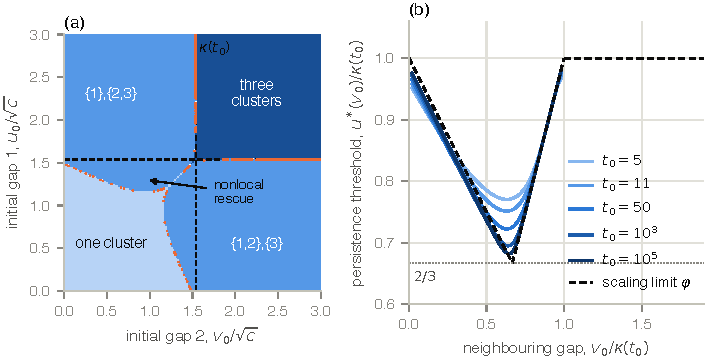
\includegraphics[width=\linewidth]{figures/fig1_phase.pdf}
\caption{\textbf{Nonlocal rescue in the three-layer chain.}
(a)~Certified limiting partition at $t_0=11$ on a $240\times240$ grid of initial gaps $(u_0,v_0)$, in units of $\sqrt c$.
Shades give the number of final clusters. Orange dots mark the 208 grid points (0.36\%) that the validated computation
did not resolve; they lie on phase boundaries. Dashed lines mark the isolated-pair threshold $\kappa(11)\approx1.539$.
Below the horizontal line, gap~1 would merge if it were isolated. In the bulge it persists, because gap~2 closes first and
pulls layer~2 away (\cref{thm:rescue}).
(b)~Normalised persistence threshold $u^*(v_0)/\kappa(t_0)$ for $t_0$ from $5$ to $10^5$ (light to dark; float estimates), shown for
$v_0<\kappa(t_0)$, together with the scaling limit $\varphi$ of \cref{thm:rescue}(c). The minimum approaches $2/3$.}
\label{fig:phase}
\end{figure}

%=====================================================================
\section{Related work}\label{sec:related}
%=====================================================================

\paragraph{Oversmoothing and attention.}
Oversmoothing of graph convolutions is exponential in depth~\citep{li2018,oono2020,cai2020}; see~\citet{rusch2023} for a
survey. \citet{wu2023} proved that graph attention with a fixed temperature also oversmooths. \citet{ma2025} characterise
when attention helps over convolution (structure noise versus feature noise); our noisy-feature regime, in which PairNorm is the best model
from depth 32 on, agrees with their prediction that attention does not help when feature noise dominates. \citet{turan2026} obtain non-homogeneous limits from activation-induced bifurcations, a different
mechanism. \citet{zhang2026} argue that oversmoothing should be measured by the effective rank~\citep{roy2007}; we report it.
Remedies include residual and initial connections~\citep{chen2020gcnii,klicpera2019}, normalisation~\citep{zhao2020pairnorm} and
continuous diffusion~\citep{chamberlain2021}; we use them as baselines in \cref{sec:downstream}.

\paragraph{Clustering in attention dynamics.}
\citet{geshkovski2023} showed that self-attention dynamics on the sphere cluster. Clusters are metastable and merge after
exponentially long times~\citep{geshkovski2024metastable,bruno2025}; causal masking changes the limit~\citep{karagodin2024}.
\citet{gao2026} report an attention-condensation transition above a sharpness threshold. These works study transformers at a
fixed inverse temperature without a graph. Our cooling schedule turns metastable clusters into permanent ones, and the graph
supplies the topology whose effect we quantify. \citet{brody2022} showed that GAT computes static attention, in which the ranking of keys
does not depend on the query; \cref{rem:gat} gives a dynamical consequence.

\paragraph{Bounded confidence and consensus.}
In the Hegselmann--Krause model~\citep{hegselmann2002} agents average only over neighbours within a confidence radius $R$.
Limiting clusters are at least $R$ apart~\citep{blondel2009}, compactly supported kernels give local
consensus~\citep{jabin2014,motsch2014}, and whether two groups merge can depend on agents between them: mediator agents, equally
spaced agents and the $2R$ conjecture~\citep{slanina2011,hegarty2014,wang2017}. Our \cref{prop:dichotomy} is the soft-kernel,
cooled analogue of the separation fact. Our rescue law is a quantitative counterpart of the qualitative mediator phenomenon: we
did not find an exact rescue boundary in this literature. Merging along edges with non-summable weights is the infinite-flow
theorem of \citet{touri2014}. The cut-balanced theorem of \citet{hendrickx2013} does not apply in discrete time here, because the
attention weights are not bounded below.

\paragraph{Annealing.}
For simulated annealing with $T_t=c/\log t$, \citet{hajek1988} showed convergence to global minima iff $c$ is at least the depth of the
deepest non-global well, through the same summability dichotomy. The leading-order $\sqrt c$ threshold is therefore classical. The
exact finite-$t_0$ law, the jump, the critical curve and the topology correction are not covered by these results.

\paragraph{Bounded confidence and temperature as architectures.}
Hegselmann--Krause-style message passing has been proposed to mitigate oversmoothing~\citep{zhou2026odnet,wang2025bimp}, and learnable
attention temperatures exist~\citep{ma2026gated}. We do not propose cooled Gaussian attention as a new architecture. We use it as the
analysable model in which cluster formation can be predicted, and we test in \cref{sec:downstream} where it helps and where it does not.

%=====================================================================
\section{Setup}\label{sec:setup}
%=====================================================================

\paragraph{Model.} Let $G=(V,E)$ be a finite undirected graph with a self-loop at every node, $N[i]$ the closed neighbourhood of
$i$ and $\Nmax=\max_i|N[i]|$. Node features $h_i(t)\in\R^p$ evolve by
\begin{equation}\label{eq:model}
h_i(t+1)=\sum_{j\in N[i]}\alpha_{ij}(t)\,h_j(t),\qquad
\alpha_{ij}(t)=\frac{\exp\big(-\|W(h_i(t)-h_j(t))\|^2/T_t\big)}{\sum_{k\in N[i]}\exp\big(-\|W(h_i(t)-h_k(t))\|^2/T_t\big)} .
\end{equation}
This is the propagation core of a deep attention GNN: one shared scoring rule, no value matrix and no nonlinearity, as in
oversmoothing analyses~\citep{wu2023,geshkovski2023}. The metric $W\in\R^{q\times p}$ is fixed (learned, in \cref{sec:prediction}).

\begin{remark}[the metric is absorbed]\label{rem:metric}
Let $z_i=Wh_i$. Then $z_i(t+1)=\sum_j\alpha_{ij}(t)z_j(t)$ with $\alpha$ computed from $\|z_i-z_j\|$, so $z$ follows
\eqref{eq:model} with $W=I$, and every result below applies to $z$. The values $h$ use the same weights. By
\cref{prop:dichotomy}, edges whose $z$-endpoints merge have non-summable weights, so their $h$-endpoints merge as well. Edges whose
$z$-endpoints stay apart have $W(h_i^\infty-h_j^\infty)\ne0$. Hence \emph{the limiting partition of $h$ equals that of $z$}, and a
learned metric decides which distinctions survive only through the distances $\|W(h_i-h_j)\|$.
\end{remark}

\paragraph{Temperature.} With a constant temperature the dynamics oversmooths.

\begin{proposition}[constant temperature]\label{prop:constT}
If $G$ is connected and $T_t\equiv T>0$, then all $h_i(t)$ converge to a common limit, exponentially fast.
\end{proposition}

We therefore study logarithmic cooling $T_t=c/\log(t+t_0)$ with $c>0$ and $t_0>1$ (our graph experiments use $t_0=|V|+2$). We
measure lengths in units of $\sqrt c$ and write $s_t:=t+t_0$. With $W=I$ the unnormalised weights become
\begin{equation}\label{eq:weights}
w_{ij}(t)=s_t^{-\|z_i(t)-z_j(t)\|^2},\qquad \alpha_{ij}=w_{ij}/\pi_i,\qquad \pi_i=\sum_{k\in N[i]}w_{ik}\in[1,\Nmax].
\end{equation}
Since $\sum_t s_t^{-d^2}$ diverges iff $d\le1$, a gap that stays below $1$ is forced to close, and a gap that stays above $1$ sees
summable attention. The difficulty is that gaps move. An edge \emph{merges} if $\|z_i-z_j\|\to0$ and \emph{persists} if its
length has a positive $\liminf$.

\paragraph{Two-block graphs.} A graph with vertex partition $V=A\sqcup B$ is \emph{block-regular} if every node of $A$ has exactly
$k_A$ closed neighbours in $A$ and $e_A\ge1$ neighbours in $B$, and symmetrically for $B$. Its \emph{cut ratios} are
$\rho_A=e_A/k_A$ and $\rho_B=e_B/k_B$. We write $\lambda=\rho_A+\rho_B$, $P=\rho_A\rho_B$, and assume $P\le1$. Examples: two
layers of the layered graph below ($\rho_A=\rho_B=1$); two $k$-cliques joined by a perfect matching ($\rho=1/k$).

\begin{lemma}[two-block reduction]\label{lem:reduction}
On a block-regular graph, block-constant features stay block-constant, and the gap $d_t=\|z_A(t)-z_B(t)\|$ obeys
\begin{equation}\label{eq:twoblock}
d_{t+1}=F_t(d_t):=d_t\,\psi(a_t),\qquad \psi(a)=\frac{1-Pa^2}{(1+\rho_Aa)(1+\rho_Ba)},\qquad a_t=s_t^{-d_t^2}.
\end{equation}
For $\rho_A=\rho_B=1$ this is $d'=d\,(1-a)/(1+a)$.
\end{lemma}

\paragraph{Layered chains.} The layered graph $G_{r,m}$ has $r$ layers of $m$ nodes. Each layer is a clique, consecutive layers are
completely joined, and there are no other edges. With scalar, layer-constant, ordered features $x_1\le\dots\le x_r$, the gaps
$g_l=x_{l+1}-x_l$ ($1\le l<r$) obey, with $w_l=s_t^{-g_l^2}$, $w_0=w_r=0$, $D_l=1+w_{l-1}+w_l$, $A=1+w_{l-1}$ and $B=1+w_{l+1}$,
\begin{equation}\label{eq:chain}
g_l'=g_l\,\frac{AB-w_l^2}{D_lD_{l+1}}+\frac{w_{l+1}g_{l+1}}{D_{l+1}}+\frac{w_{l-1}g_{l-1}}{D_l}.
\end{equation}
All three terms are nonnegative. The first is the isolated two-layer map with extra damping; the other two are pushes from the
neighbouring gaps.

\paragraph{Validated numerics.} Several results are computer-assisted. We evaluate \eqref{eq:twoblock} and \eqref{eq:chain} in
interval arithmetic~\citep{tucker2011} and stop as soon as an analytic certificate proves the fate of every gap
(\cref{app:numerics}). Persistence is certified by a tail bound (certificate C1, \cref{thm:two-block}(vi)), merging by a block-diameter
bound (C2). Statements called \emph{proved} use \texttt{mpmath} interval arithmetic at 160 bits~\citep{mpmath}. Statements called
\emph{certified} use float64 intervals with outward rounding, where $\exp$ and $\log$ are padded by 4 ulp; they are rigorous provided the
platform's elementary functions are accurate to 4 ulp.

%=====================================================================
\section{Two blocks: an exact threshold law}\label{sec:twoblock}
%=====================================================================

\begin{theorem}[two-block law]\label{thm:two-block}
Let $\rho_A,\rho_B>0$ with $P=\rho_A\rho_B\le1$, $t_0>1$, and let $d_t$ follow \eqref{eq:twoblock} from $d_0>0$.
\begin{enumerate}[label=(\roman*),leftmargin=2em,itemsep=1pt]
\item \emph{Dichotomy.} $d_\infty=\lim_td_t$ exists and $d_\infty\in\{0\}\cup[1,\infty)$. Moreover $d_\infty=0$ iff $d_T\le1$ for some $T$.
\item \emph{Threshold.} There is $\kappa=\kappa(t_0;\rho_A,\rho_B)\in(1,\infty)$ such that the gap merges iff $d_0<\kappa$.
\item \emph{First-order jump.} $d_0\mapsto d_\infty$ is nondecreasing and right-continuous, and $d_\infty(\kappa)=1$. The limiting gap
jumps from $0$ to exactly $\sqrt c$ at the threshold.
\item \emph{Critical curve and monotonicity.} $\kappa(t_0+k)=F_{k-1}\circ\dots\circ F_0(\kappa(t_0))$ for $k\in\N$. Moreover $\kappa$ is
nonincreasing in $t_0$ and nondecreasing in $\rho_A$ and in $\rho_B$.
\item \emph{Second-order asymptotics.} For fixed $\rho_A,\rho_B$, with $L=\log t_0\to\infty$,
\[
\kappa(t_0;\rho_A,\rho_B)=1+\frac{\log L-\frac12\log\log L+\frac12\log(\rho_A+\rho_B)+o(1)}{L}.
\]
Equivalently, in physical units with initial temperature $T_0=c/\log t_0$, the critical gap $d_{\rm crit}$ satisfies
$d_{\rm crit}^2=c+T_0\big[2\log\frac c{T_0}-\log\log\frac c{T_0}+\log(\rho_A+\rho_B)+o(1)\big]$ as $T_0\to0$.
\item \emph{Explicit bounds.} $\kappa(t_0)\ge1+\varepsilon_-$, where $\varepsilon_-$ is the unique root of
$\varepsilon(2\varepsilon+\varepsilon^2)=\lambda_-\,t_0^{-(2\varepsilon+\varepsilon^2)}$ and
$\lambda_-=\sum_{X\in\{A,B\}}\rho_X/(1+\rho_X/t_0)$. Conversely (certificate C1), if $1<\delta<d_0$ and
\begin{equation}\label{eq:C1}
\log d_0-\Lambda_\delta\,\frac{(t_0-1)^{1-\delta^2}}{\delta^2-1}\ \ge\ \log\delta,\qquad
\Lambda_\delta=\lambda+\frac{Pq}{1-Pq^2},\quad q=t_0^{-\delta^2},
\end{equation}
then $d_t\ge\delta$ for all $t$, so $\kappa(t_0)\le d_0$.
\end{enumerate}
\end{theorem}

The proof is in \cref{app:twoblock}. Part~(i) is the soft-kernel analogue of the bounded-confidence separation
fact~\citep{blondel2009}, and the limit $\kappa\to1$ in part~(v) is Hajek's summability criterion~\citep{hajek1988}. The new content is
(ii)--(vi) at finite $t_0$ and the expansion in (v), whose error is $o(1/\log t_0)$. The proof of (v) compares the trajectory with explicit barriers
$1+X(\log s_t)$, $X(\tau)=(\log\tau-\frac12\log\log\tau+\frac12\log\lambda\pm\eta)/\tau$: with $+\eta$ the map cannot cross the barrier
from above, with $-\eta$ it cannot cross from below, and below the lower barrier the accumulated attention exceeds the available gap. In
physical units the effective confidence radius is $\sqrt c\,\kappa(t_0)$, not $\sqrt c$. The excess $d_{\rm crit}^2-c\approx2T_0\log(c/T_0)$
is the distance that a gap loses before its own weight becomes summable. The correction is large in practice: $\kappa(11)\in[1.53858,1.53909]$, so at $t_0=11$ a gap must be $54\%$ above
$\sqrt c$ to survive (\cref{tab:kappa}). \Cref{fig:twoblock} shows the enclosures, the jump and the critical slowing down implied by (iii)
and (iv). Trajectories started just above $\kappa$ follow the critical curve for up to $10^6$ layers before they settle or merge.

\begin{corollary}[topology enters at second order]\label{cor:topology}
For fixed cut ratios with sums $\lambda=\rho_A+\rho_B$ and $\lambda'=\rho_A'+\rho_B'$,
\[
\kappa(t_0;\rho_A,\rho_B)-\kappa(t_0;\rho_A',\rho_B')=\frac{\frac12\log(\lambda/\lambda')+o(1)}{\log t_0}.
\]
In physical units the critical squared gap shifts by $T_0\log(\lambda/\lambda')+o(T_0)$. The product $P=\rho_A\rho_B$ does not enter at this
order.
\end{corollary}

The reading is an energy--entropy balance. A gap $d$ shrinks at relative rate $\approx\lambda\,e^{-d^2/T_t}$, so multiplying the cut ratios by
a factor is equivalent to shifting $d^2$ by $T_t$ times its logarithm. Topology matters at finite depth: $\kappa(11)$ ranges from $1.30$ for
$\rho_A=\rho_B=0.1$ to $1.54$ for $\rho_A=\rho_B=1$ (\cref{tab:rho}). The $o(1)$ term converges slowly when $\lambda$ is small.

\begin{proposition}[third term]\label{prop:third}
For fixed $\rho_A,\rho_B$, with $\lambda=\rho_A+\rho_B$ and $L=\log t_0\to\infty$,
\[
\kappa(t_0;\rho_A,\rho_B)=1+\frac1L\Big[\log L-\tfrac12\log\log L+\tfrac12\log\lambda+\frac{\log\log L-\log\lambda+2+o(1)}{4\log L}\Big].
\]
In particular, the topology shift of \cref{cor:topology} is $\frac{\log(\lambda/\lambda')}{2L}\big(1-\frac1{2\log L}\big)+o\big(\frac1{L\log L}\big)$.
\end{proposition}

The proof (\cref{app:second}) uses the barriers of (v) with $c$ replaced by
$\frac12\log\lambda+(\log\log\tau-\log\lambda+2\pm\eta)/(4\log\tau)$.
At this order the $\pm\eta$ term decides the sign of every comparison, including the summation that rules out persistence below the
lower barrier. The topology shift therefore approaches its limit only like $1-1/(2\log\log t_0)$, which is why it converges so slowly in
\cref{fig:twoblock}(b).

\begin{remark}[accuracy at finite $t_0$]\label{rem:second}
For $\lambda=2$ the two-term formula of (v) is already accurate at moderate $t_0$: it lies below the validated enclosures by at most
$0.05/\log t_0$ for $17\le t_0\le10^4$ (\cref{tab:kappa}). For smaller $\lambda$ the third term is larger and the two-term formula converges
more slowly (\cref{tab:residual}). Adding the third term reduces the residual by an order of magnitude for $L\gtrsim10^3$, while at small $L$
it overcorrects. The root $\varepsilon_-$ in (vi) has $-\log\log L$ instead of $-\frac12\log\log L$ in its expansion: the bound
freezes the gap, while the true gap shrinks along the critical curve, and this costs the extra $\frac12\log\log L/L$.
\end{remark}

\begin{figure}[t]
\centering
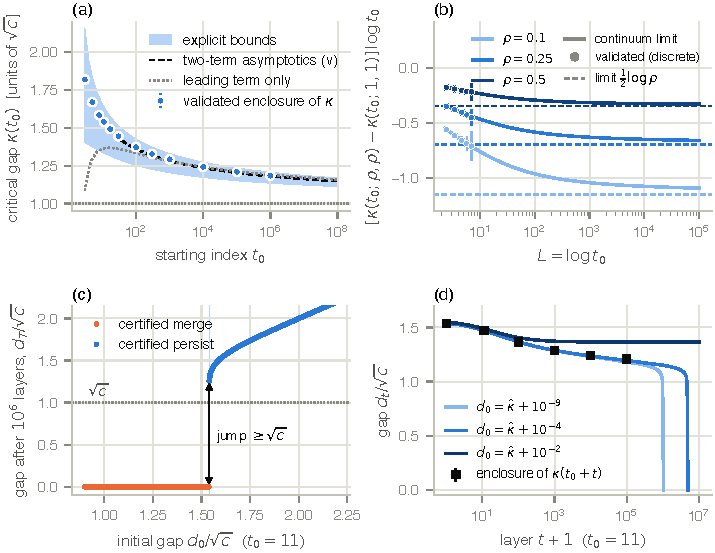
\includegraphics[width=\linewidth]{figures/fig2_two_block.pdf}
\caption{\textbf{The two-block law (\cref{thm:two-block}).}
(a)~Validated enclosures of $\kappa(t_0)$ for $\rho_A=\rho_B=1$ (dots; widths below $0.05$), the explicit bounds of part~(vi) (band),
the two-term asymptotics of part~(v) (dashed) and its leading term alone (dotted).
(b)~Topology at second order (\cref{cor:topology}): the threshold shift relative to $\rho=1$, multiplied by $\log t_0$, tends to
$\frac12\log\rho$ (dashed). Dots: validated enclosures of the discrete map ($t_0\le10^3$); lines: continuum limit up to $t_0=e^{10^5}$. The
approach is slow, with relative error $\approx1/(2\log\log t_0)$ (\cref{prop:third}).
(c)~Gap after $10^6$ layers against the initial gap at $t_0=11$. Every point is certified to merge (orange) or to persist (blue). The
gap jumps from $0$ to at least $\sqrt c$ at $\kappa$ (shaded, width $5\cdot10^{-4}$).
(d)~Critical slowing down. Trajectories started just above the float estimate $\hat\kappa$ of $\kappa(11)$ follow the critical curve
$\kappa(t_0+t)$ (squares: validated enclosures, part~(iv)) for up to $10^6$ layers.}
\label{fig:twoblock}
\end{figure}

%=====================================================================
\section{Chains: one-sided errors and nonlocal rescue}\label{sec:chains}
%=====================================================================

Let $F_t$ denote the isolated two-layer map ($\rho_A=\rho_B=1$) and $\kappa(t_0)=\kappa(t_0;1,1)$.

\begin{lemma}[comparison]\label{lem:comparison}
Along \eqref{eq:chain} all gaps stay nonnegative and $g_l(t+1)\ge F_t(g_l(t))$ for every $l$ and $t$.
\end{lemma}

The neighbouring gaps can only push a gap open. This has three consequences.

\begin{theorem}[one-sided errors]\label{thm:chain}
Consider $G_{r,m}$ with ordered layer-constant features.
\begin{enumerate}[label=(\alph*),leftmargin=2em,itemsep=1pt]
\item If $g_l(t_1)\ge\kappa(t_0+t_1)$ for some $t_1$, then $g_l(t)\ge1$ for all $t\ge t_1$; the gap persists.
\item The isolated-pair rule ``gap $l$ persists iff $g_l(0)\ge\kappa(t_0)$'' never predicts persistence for a gap that merges. All of
its errors are \emph{rescues}: gaps below $\kappa(t_0)$ that persist.
\item The early-depth rule $\mathcal R_{t_1}$: ``gap $l$ persists iff $g_l(t_1)\ge\kappa(t_0+t_1)$'' has the same one-sided error. The set
of gaps it declares persistent is nondecreasing in $t_1$. Every gap with $\lim_tg_l(t)\ne1$ is classified correctly for all large $t_1$.
\end{enumerate}
\end{theorem}

The early-depth rule needs only $t_1$ layers of forward computation and the scalar function $\kappa$, which we tabulate once.
\Cref{sec:prediction} shows that it is accurate already at $t_1=10$.

\paragraph{Three layers.} We now quantify the rescue. Write $u=g_1$, $v=g_2$ for the two gaps of $G_{3,m}$ and $h=u+v/2$, the distance
from layer~1 to the midpoint of layers~2 and~3. The \emph{rescue boundary} $u^*(v_0)$ is the smallest $u_0$ from which gap~1
persists; we define the upper and lower versions $U_\pm$ in \cref{app:three}.

\begin{theorem}[nonlocal rescue law]\label{thm:rescue}
Let $t_0\ge2$.
\begin{enumerate}[label=(\alph*),leftmargin=2em,itemsep=1pt]
\item \emph{Exact criterion.} Gap~1 merges whenever $u_0+v_0/2<1$. If $u_0+v_0<2$, gap~1 persists iff $h(t)\ge1$ for all $t$; in that
case layers 2 and 3 merge and gap~1 converges to $\lim_th(t)$. On the symmetric line $u_0=v_0<1$ both gaps merge.
\item \emph{Rescue at every $t_0$.} For every $v_0>0$ there is an explicit $R(t_0,v_0)>0$ such that gap~1 persists for every
$u_0\ge\kappa(t_0)-R$. The isolated rule is wrong on $[\kappa-R,\kappa)$; the neighbour pushes $u$ across the critical curve in one step.
\item \emph{Scaling limit.} Let $\varphi(x)=\max\{x,1-x/2\}$ for $0<x<1$ and $\varphi(x)=1$ for $x>1$. For every $x\in(0,1)\cup(1,\infty)$,
\[
\lim_{t_0\to\infty}\frac{U_\pm(x\,\kappa(t_0);t_0)}{\kappa(t_0)}=\varphi(x),\qquad
\lim_{t_0\to\infty}\inf_{v_0>0}\frac{U_\pm(v_0;t_0)}{\kappa(t_0)}=\varphi\big(\tfrac23\big)=\tfrac23 .
\]
\end{enumerate}
\end{theorem}

The limit $\varphi$ has a simple reading. If the neighbouring gap is small ($x<2/3$), it closes first, and layer~1 then faces the merged
pair at distance $h=u+v/2$: gap~1 survives iff $h$ clears the threshold, giving $1-x/2$. If $2/3<x<1$, the two gaps race and the larger
one survives ($\varphi=x$). If $x>1$, the neighbour persists itself and does not help ($\varphi=1$). Rescue is strongest at $x=2/3$, where a
gap one third below the isolated threshold still survives. At finite $t_0$ the minimum is $0.770,0.751,0.722,0.695,0.682$ for
$t_0=5,11,50,10^3,10^5$ (\cref{fig:phase}b). The constant $T^*$ beyond which (c) applies is explicit but huge near the corner $x=2/3$, so
for moderate $t_0$ we rely on computer-assisted proofs.

\begin{theorem}[computer-assisted, $t_0=11$]\label{thm:cap}
\begin{enumerate}[label=(\alph*),leftmargin=2em,itemsep=1pt]
\item (proved) $1.538<\kappa(11)<1.540$.
\item (proved) The six initial conditions in \cref{tab:rigorous} have the stated limiting partitions. In particular, at $u_0=1.4<\kappa(11)$
the fate of gap~1 is not monotone in $v_0$: it merges for $v_0=0.1$, persists for $v_0\in\{0.5,0.95\}$ and merges for
$v_0\in\{1.5,3.0\}$. Also $u_0=1.2$, $22\%$ below $\kappa(11)$, persists for $v_0=0.95$, and $v_0=1.5<\kappa(11)$ persists for $u_0=1.4$.
\item (certified) On the grid $\{0.0125,0.025,\dots,3\}^2$, $57{,}392$ of $57{,}600$ initial conditions (99.64\%) have a certified
limiting partition (\cref{fig:phase}a). The smallest certified persisting gap is $u_0=1.1625$ ($24\%$ below $\kappa(11)$), at
$v_0=0.8875$. No column of the grid has a non-monotone fate in $u_0$.
\end{enumerate}
\end{theorem}

%=====================================================================
\section{General graphs: dichotomy and planted partitions}\label{sec:graphs}
%=====================================================================

We now return to \eqref{eq:model} on an arbitrary graph with vector features ($W=I$ by \cref{rem:metric}).

\begin{proposition}[universal dichotomy]\label{prop:dichotomy}
For every graph with self-loops, every $t_0>1$ and every initial condition: (i) every $z_i(t)$ converges to some $z_i^\infty$; (ii) if
$\sum_tw_{ij}(t)=\infty$ on an edge $\{i,j\}$, then $z_i^\infty=z_j^\infty$; (iii) every limiting edge length
$\|z_i^\infty-z_j^\infty\|$ lies in $\{0\}\cup[1,\infty)$.
\end{proposition}

Limiting edge lengths in $(0,\sqrt c)$ are therefore impossible on every graph. The limiting partition is well defined: its blocks are the
connected components of the edges of length $0$. The proof applies the infinite-flow theorem of \citet{touri2014} to the attention
matrices, which have a uniformly positive diagonal and are balanced in their sense. Next, let $V=B_1\sqcup\dots\sqcup B_K$ be a planted
partition. Blocks $k\neq l$ are \emph{adjacent} ($k\sim l$) if an edge joins them, $e_{\max}$ is the largest number of neighbours a node has
outside its block, and $C_k\supseteq\{z_i(0):i\in B_k\}$ is convex with diameter $D_k$.

\begin{theorem}[planted partitions at the $\sqrt c$ scale]\label{thm:planted}
Let $t_0\ge2$, let each $G[B_k]$ be connected, and let $\eta\ge0$ and $\delta>1$ satisfy
\[
\text{(A1)}\ \ D_k+2\eta\le1\ \ \forall k,\qquad
\text{(A2)}\ \ \dist(C_k,C_l)\ge\delta+2\eta\ \ \forall k\sim l,
\]
\[
\text{(A3)}\ \ e_{\max}\,\delta\,\frac{(t_0-1)^{1-\delta^2}}{\delta^2-1}\le\eta .
\]
Then $z_i(t)\in C_k+\bar B(\eta)$ for all $t$ and $i\in B_k$. Each block converges to a single point $z_k^\infty$, adjacent blocks end at
distance $\ge\delta$, and the limiting partition is exactly $\{B_1,\dots,B_K\}$.
\end{theorem}

\begin{corollary}[ball form and leading-order sharpness]\label{cor:planted}
(a) If block $k$ lies in a ball of radius $r_k$ around $\mu_k$, it suffices that $r_k\le\frac12-\eta$ and
$\|\mu_k-\mu_l\|\ge r_k+r_l+\delta+2\eta$ for $k\sim l$, with (A3). In physical units: $r\le\sqrt c\,(\frac12-\eta)$ and
$\Delta\ge2r+(\delta+2\eta)\sqrt c$.
(b) Fix $e_{\max}$ and $\theta\in(0,1]$. If $D_k\le1-\theta$ and $\dist(C_k,C_l)\ge\Gamma(t_0)$ for $k\sim l$, with an explicit
$\Gamma(t_0)=1+(1+o(1))\frac{\log\log t_0}{\log t_0}$, the conclusions hold for all large $t_0$. By \cref{thm:two-block}(v), $\Gamma$ matches the
two-block threshold $\kappa(t_0;\rho_A,\rho_B)$ to leading order for every topology, and separation $\kappa(t_0;\rho_A,\rho_B)$ is necessary
for block-regular graphs with collapsed blocks. At second order $\Gamma$ is not sharp: $\Gamma-\kappa=(\frac12+o(1))\log\log\log t_0/\log t_0$.
\end{corollary}

\begin{proposition}[the diameter condition is sharp]\label{prop:sharp}
For every $D>1$ and $t_0\ge2$ there is a graph with a single connected block and initial features of diameter $D$ whose limit is not a
consensus. Hence no condition $\max_kD_k\le f(t_0)$ with $f(t_0)>1$ guarantees the planted partition on all graphs.
\end{proposition}

The construction is two large cliques joined by a perfect matching: the cut ratio $1/k$ makes the threshold of \cref{thm:two-block} drop
towards $1$. \Cref{thm:planted} removes the factor $1/(4\sqrt\rho)$ ($\rho$ the hop radius of a block) that our earlier path-product
argument required. On the noisy SBMs of \cref{sec:prediction} it certifies all 100 runs with $\sigma\le0.1$, against 28 runs for the earlier
condition. It never certifies a run in which the planted partition fails.

%=====================================================================
\section{Learned query--key attention}\label{sec:learned}
%=====================================================================

So far the score has been a squared distance. Practical attention layers score pairs with learned queries and keys. We now replace the
Gaussian score by a quadratic score with the same cooling,
\begin{equation}\label{eq:qk}
\alpha_{ij}(t)\propto\exp\big(f(z_i,z_j)\log s_t\big)\ \ (j\in N[i]),\qquad f(x,y)=x^\top Jy-\tfrac12y^\top\Omega y+b^\top y ,
\end{equation}
with $c=1$. Dot-product attention with query and key biases, $(W_Qx+q)^\top(W_Ky+k)$, is the case $J=W_Q^\top W_K$, $\Omega=0$ and
$b=W_K^\top q$; terms that depend only on the query $x$ cancel in the softmax. Gaussian attention with metric $W$ is the case $J=\Omega=2W^\top W$,
$b=0$. Because $N[i]$ contains $i$, the weights depend on $f$ only through the \emph{directed margins}
\[
m_{ij}=f(z_i,z_i)-f(z_i,z_j),\qquad w_{ij}=s_t^{-m_{ij}},\qquad \alpha_{ij}=w_{ij}/\pi_i,\qquad \pi_i={\textstyle\sum_{k\in N[i]}}w_{ik}\ge1 .
\]
The margin $m_{ij}$ is how much node $i$ prefers itself to $j$. The Gaussian margin $\|z_i-z_j\|^2$ is nonnegative and symmetric; a learned
margin is neither.

\begin{proposition}[margin decomposition]\label{prop:margin}
Let $J_s$ and $J_a$ be the symmetric and antisymmetric parts of $J$, and $\mathcal V(x)=\frac12x^\top(J_s-\Omega)x+b^\top x$. Then
\[
m_{ij}=\tfrac12(z_i-z_j)^\top J_s(z_i-z_j)+\mathcal V(z_i)-\mathcal V(z_j)-z_i^\top J_az_j,\qquad m_{ij}+m_{ji}=(z_i-z_j)^\top J_s(z_i-z_j).
\]
\end{proposition}

The attention weight is thus a Gaussian kernel in the metric $J_s/2$, times a key prior $s_t^{\mathcal V(z_j)}$, times a rotation factor. The
Gaussian model is the case in which $\mathcal V$ is constant and $J_a=0$. In dot-product attention $\mathcal V(x)=\frac12x^\top J_sx+b^\top x$, so nodes
with large keys attract their neighbours. The sum of the two margins of an edge is fixed by $J_s$ alone. The potential and the rotation only
split it between the two directions.

\paragraph{Two blocks.} On a block-regular graph, block-constant features stay block-constant for every score, and
\[
z_B'-z_A'=k\,(z_B-z_A),\qquad k=1-p_A-p_B=\frac{1-Pa_Aa_B}{(1+\rho_Aa_A)(1+\rho_Ba_B)},\qquad p_X=\frac{\rho_Xa_X}{1+\rho_Xa_X},
\]
with $a_A=s_t^{-m_{AB}}$ and $a_B=s_t^{-m_{BA}}$ (\cref{lem:reduction-learned}); for $a_A=a_B$ this is the factor $\psi$ of \cref{lem:reduction}. The
gap keeps its direction $e$, up to sign. Write $M_A=m_{AB}$, $M_B=m_{BA}$, $\sigma=e^\top J_se$ and $\omega=e^\top\Omega e/\sigma$. For the
score~\eqref{eq:qk} with $\sigma>0$ the two margins form a closed system,
\begin{equation}\label{eq:margin-map}
M_X'=k\Big[M_X-(M_A+M_B)\big(\tfrac\omega2(p_A+p_B)+(1-\omega)\,p_X\big)\Big],\qquad X\in\{A,B\},
\end{equation}
with $M_A+M_B=\sigma\|z_A-z_B\|^2$. Since $a_Aa_B=s_t^{-(M_A+M_B)}<1$, $k>0$: the blocks never cross. The fate of the pair depends on $J$, $\Omega$ and $b$ only through the two margins and $\omega$:
dot-product attention has $\omega=0$, Gaussian attention $\omega=1$.

\begin{theorem}[two blocks under learned attention]\label{thm:learned}
Let $\sigma>0$, $0\le\omega\le1$ and $P=\rho_A\rho_B\le1$.
\begin{enumerate}[label=(\roman*),leftmargin=2em,itemsep=1pt]
\item \emph{Dichotomy.} The blocks merge iff $\min(M_A,M_B)\le1$ at some layer. Otherwise both margins decrease to limits $\ge1$, and the blocks
converge to two distinct points.
\item \emph{Symmetric pairs.} If $\rho_A=\rho_B$ and $M_A=M_B$ at $t=0$, then $M_A=M_B$ for all $t$, and $\sqrt{M_A}$ follows the Gaussian map
$F_t$ of~\eqref{eq:twoblock}. Hence the pair persists iff $M_A(0)\ge\kappa(t_0;\rho_A,\rho_A)^2$, and \cref{thm:two-block} applies to
$\sqrt{M_A}$.
\item \emph{Bounds.} If the pair persists, then $\min(M_A,M_B)\ge1+\varepsilon_\omega$ at $t=0$, where $\varepsilon_\omega$ is the root of
$\varepsilon^2=(1-\frac\omega2)\rho_-t_0^{-\varepsilon}$ and $\rho_-=\min_X\rho_X/(1+\rho_X/t_0)$. Conversely (certificate C1$'$), let
$1<\delta^2<m:=\min(M_A,M_B)$, $R=(M_A+M_B)/\delta^2$, $q=t_0^{-\delta^2}$ and $R\lambda q<1$. If
\[
\log\frac m{\delta^2}\ \ge\ \frac{(1+R)\lambda}{1-R\lambda q}\cdot\frac{(t_0-1)^{1-\delta^2}}{\delta^2-1},
\]
then both margins stay above $\delta^2$ and the pair persists.
\item \emph{Leading order.} For every $\bar M$ there are $\gamma_\pm(t_0)=(2+o(1))\log\log t_0/\log t_0$ such that a pair with
$M_A+M_B\le\bar M$ merges if $\min(M_A,M_B)<1+\gamma_-$ and persists if $\min(M_A,M_B)\ge1+\gamma_+$. To leading order the critical margin is
$\kappa(t_0)^2$.
\end{enumerate}
\end{theorem}

The isolated-pair rule of \cref{sec:twoblock} therefore carries over with one change: the squared gap is replaced by the smaller of the two
directed margins. A pair is lost through its weaker direction. Since $\min(M_A,M_B)\le\frac12(M_A+M_B)=\frac12\sigma\|z_A-z_B\|^2$, with equality
iff the potential and the rotation cancel on the pair, the symmetric pairs of (ii) are the most robust. For a fixed symmetric part $J_s$, key biases,
key norms and rotations can only make a pair merge earlier, to leading order. Beyond leading order the critical value of the weaker margin
depends on the partner margin. In units of $\kappa(t_0)^2$ it lies between $0.92$ and $1.07$ for partner margins up to $10$, at $t_0=11$ and
$t_0=10^3$ and for $\omega\in\{0,1\}$ (\cref{fig:learned}a). At every computed point the two critical margins sum to more than
$2\kappa(t_0)^2$. So at a fixed gap the symmetric split is also the most robust one at finite $t_0$, as far as we computed.

\paragraph{What does not carry over.} Two properties of the Gaussian dynamics fail for learned scores.

\begin{proposition}[oscillation]\label{prop:oscillation}
Let $f(x,y)=x^\top Jy$ and $\rho_A=\rho_B=\rho\ge1$, and let the blocks start at $z_A=-z_B$ with $\sigma=e^\top J_se<0$. Then $z_A(t)=-z_B(t)$
for all $t$, and $D_t=(|\sigma|/2)^{1/2}\|z_A(t)-z_B(t)\|$ follows the Gaussian map $F_t$ with cut ratios $(1/\rho,1/\rho)$. If
$D_0\ge\kappa(t_0;1/\rho,1/\rho)$, the blocks exchange sides at every layer and $D_t\to D_\infty\ge1$, so the features never converge, although
the attention between the blocks is not summable. Otherwise the blocks merge.
\end{proposition}

A score whose symmetric part is negative along a direction makes nodes prefer neighbours that differ along it, as a heterophilous attention
head would. Under cooling such a head turns a two-block structure into a period-two oscillation, and both convergence and part~(ii) of
\cref{prop:dichotomy} fail. GAT~\citep{velickovic2018} fails in a different way. Its score $\mathrm{LeakyReLU}(u^\top x+v^\top y)$ gives
$|m_{ij}+m_{ji}|\le(1-\beta)\min(|u^\top(z_i-z_j)|,|v^\top(z_i-z_j)|)$, where $\beta$ is the negative slope, and $m_{ij}=-m_{ji}$ when the four
arguments of the edge share a sign (\cref{rem:gat}). In that regime one block of a pair has a nonpositive margin, and the gap shrinks by a fixed
factor at every layer. This is the dynamical side of the static attention of GAT~\citep{brody2022}.

\paragraph{General graphs.} The separation half of \cref{thm:planted} holds for every score
(\cref{prop:separation}). If the directed margins between adjacent blocks are at least $\delta^2$ on the $\eta$-neighbourhoods of their hulls,
and $e_{\max}R\,(t_0-1)^{1-\delta^2}/(\delta^2-1)\le\eta$ with $R$ the largest diameter of the union of two such neighbourhoods, then every block
stays in its neighbourhood and no two adjacent blocks merge. The in-block half of \cref{thm:planted} and \cref{prop:dichotomy} rest on the
symmetry of the weights, through the cut balance of \citet{touri2014}. Whether the features converge and the limiting partition consists of the components of
zero-length edges when $J_s\succ0$ is open. For prediction, we use the margin to the best neighbour,
$m^+_{ij}=\max_{k\in N[i]}f(z_i,z_k)-f(z_i,z_j)\ge m_{ij}$, which sets the weight up to a bounded factor: $s_t^{-m^+_{ij}}/\Nmax\le\alpha_{ij}\le
s_t^{-m^+_{ij}}$. The \emph{directed threshold-graph rule} returns the components of the edges with $\min(m^+_{ij},m^+_{ji})<\kappa(t_0+t_1)^2$.
For Gaussian attention it is the rule of \cref{sec:prediction}. On two blocks it is the leading-order rule of \cref{thm:learned}.

\begin{figure}[t]
\centering
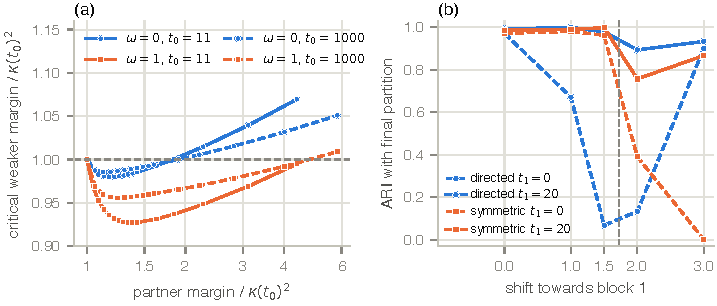
\includegraphics[width=\linewidth]{figures/fig7_learned.pdf}
\caption{\textbf{Learned attention} (E9). (a)~Critical value of the weaker margin of a two-block pair against the partner margin, both in
units of $\kappa(t_0)^2$, for dot-product ($\omega=0$) and Gaussian-type ($\omega=1$) scores ($\rho_A=\rho_B=1$; float bisection with the merge test of
\cref{thm:learned}(i) and certificate C1$'$). The diagonal point is exact by \cref{thm:learned}(ii). (b)~Contextual SBMs under dot-product attention, with all features shifted towards
block~1 (30 runs per shift). ARI between the final partition and the directed rule, or the rule that uses only the symmetric part
$\frac12(m_{ij}+m_{ji})$, applied after $t_1$ layers. Dashed vertical line: shift at which the margin between block means equals $\kappa(t_0)^2$.}
\label{fig:learned}
\end{figure}

\paragraph{Contextual SBMs (E9).} We test the directed rule on the SBMs of E4 (four blocks, $p_{\rm out}=0.01$, $\sigma\in\{0.1,0.2,0.3\}$) under
dot-product attention $f(x,y)=x^\top Jy$, with tied ($J=2I$) or untied queries and keys (\cref{app:exp}). With $J_s=2I$ the symmetric part of
every margin is the squared distance of E4, so a rule that sees only $\frac12(m_{ij}+m_{ji})$ is the Gaussian rule. To create a key potential we
shift all features by $\nu$ towards block~1. At the block means the margin of every other block towards block~1 then drops from $9$ to
$9-3\sqrt2\,\nu$, and the reverse margins grow by the same amount. The other blocks are absorbed into block~1 in 29 of 30 runs at $\nu=3$ and in
part of the runs at $\nu=2$. The symmetric rule cannot see this: applied to the initial features, it predicts at least four clusters at every shift
(\cref{fig:learned}b). Applied after
$t_1=20$ layers, the directed rule recovers the final partition with mean ARI $0.91$ at $\nu\ge2$, against $0.81$ for the symmetric rule, and both
reach $0.99$ at $\nu\le1.5$. In 7 of the 10 runs where its ARI is below $0.9$, the directed rule predicts fewer clusters than form.

At $t_1=0$ the directed rule over-merges. Its errors are one-sided: in 148 of the 150 runs no edge that it predicts to persist ends merged.
The symmetric rule wrongly predicts persistence for some edges in 83 runs. The cause is that a learned margin is first order in the feature noise, through
$\mathcal V(z_i)-\mathcal V(z_j)$, while the squared distance is second order. Before the blocks contract, a few cross edges of a well-separated pair
fall below the threshold, and one such edge joins two predicted components. Five layers remove most of these errors: the mean ARI over all runs
is $0.55$, $0.93$ and $0.96$ at $t_1=0,5,20$. Blocks also contract towards their high-potential members before they interact, so the
block-mean margin is only a rough guide: at $\nu=2$ it is $0.51$, below $\kappa^2\approx1.69$, yet most runs end with two to five clusters. No run
oscillates, as expected for $J_s\succ0$: the largest change in the last layer is $4\cdot10^{-4}$. \Cref{sec:downstream} tests the rule on trained
dot-product networks.

%=====================================================================
\section{Predicting clusters}\label{sec:prediction}
%=====================================================================

\begin{figure}[!t]
\centering
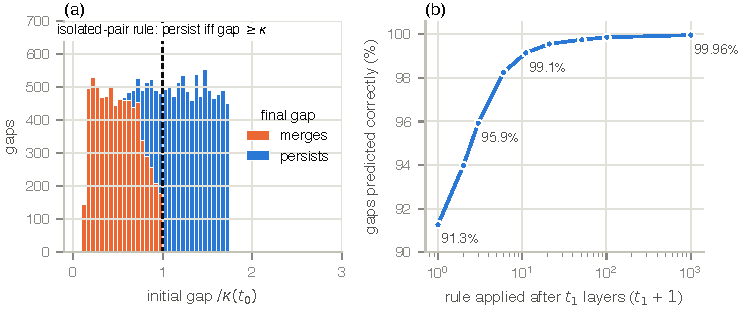
\includegraphics[width=\linewidth]{figures/fig3_chains.pdf}
\caption{\textbf{Five-layer chains} ($t_0=17$; 3972 certified random initial conditions; 15,888 gaps).
(a)~Initial gaps, stacked by final fate. No gap at or above $\kappa(t_0)$ merges (\cref{thm:chain}). Every error of the isolated rule is a
rescued gap below $\kappa$, down to $0.53\,\kappa$.
(b)~Accuracy of the early-depth rule $\mathcal R_{t_1}$ against $t_1$. By \cref{thm:chain}(c) it can only improve with $t_1$.}
\label{fig:chains}
\end{figure}

\begin{figure}[!t]
\centering
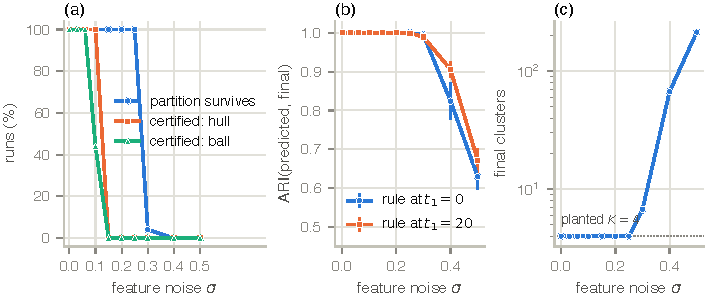
\includegraphics[width=\linewidth]{figures/fig4_sbm.pdf}
\caption{\textbf{Noisy contextual SBMs} ($K=4$ blocks of 150 nodes, $p=8$, block means $3\sqrt c$ apart, $t_0=602$, 4000 layers; 25 runs
per $\sigma$).
(a)~Runs in which the planted partition survives, and runs certified by \cref{thm:planted} (hull form) and by \cref{cor:planted}(a) (ball form).
(b)~ARI between the threshold-graph prediction and the final partition, with the rule applied at $t_1=0$ or after $t_1=20$ layers
(mean $\pm$ 95\% CI).
(c)~Number of final clusters (mean $\pm$ 95\% CI).}
\label{fig:sbm}
\end{figure}

\begin{figure}[!t]
\centering
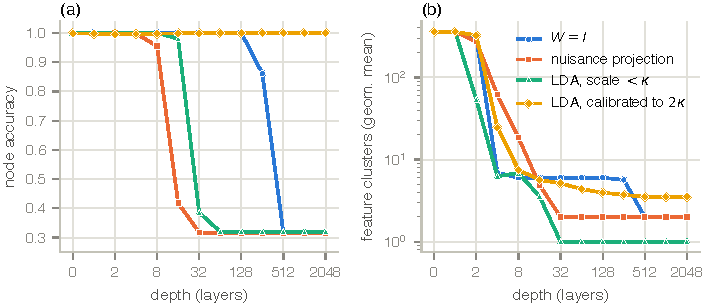
\includegraphics[width=\linewidth]{figures/fig5_metric.pdf}
\caption{\textbf{A learned metric decides which distinctions survive} (5 seeds). Attention uses $z=Wh$, values are $h$.
(a)~Linear-probe accuracy against depth. (b)~Number of final feature clusters (geometric mean over seeds).
Only the metric that places the class distinctions above the threshold keeps the classes to depth 2048.}
\label{fig:metric}
\end{figure}

The theory suggests one prediction rule at three levels of generality. For chains, $\mathcal R_{t_1}$ thresholds every gap at
$\kappa(t_0+t_1)$ after $t_1$ layers (\cref{thm:chain}). For general graphs, the \emph{threshold-graph rule} runs $t_1$ layers and returns the
connected components of the edges with $\|z_i(t_1)-z_j(t_1)\|<\kappa(t_0+t_1)$, using the two-layer $\kappa$. By
\cref{prop:dichotomy} the true limiting partition consists of the components of zero-length edges. We test the rules against long runs
(\cref{app:exp}).

\paragraph{Five-layer chains (E3).} We draw 4000 random gap vectors of $G_{5,m}$ with gaps uniform in $[0.2,2.6]$ at $t_0=17$
($\kappa\in[1.4908,1.4916]$) and certify the limiting partition of 3972 of them. The isolated rule classifies $91.3\%$ of the $15{,}888$ gaps
and $68.0\%$ of the partitions correctly. It never predicts persistence wrongly, as \cref{thm:chain}(b) requires. All $1387$ errors are
rescues, the smallest at $u_0=0.79$, below $\sqrt c$ (\cref{fig:chains}a). The early-depth rule removes most of them: it is correct for
$94.0\%$, $98.3\%$, $99.1\%$ and $99.96\%$ of the gaps at $t_1=1,5,10$ and $1000$ (\cref{fig:chains}b).

\paragraph{Noisy community graphs (E4).} We use $K=4$ SBM blocks of 150 nodes ($p_{\rm in}=0.2$, $p_{\rm out}\in\{0,0.005,0.01,0.02,0.05\}$),
features in $\R^8$ with block means at mutual distance $3\sqrt c$ plus isotropic noise $\sigma$, and $t_0=|V|+2=602$, where $\kappa\approx1.301$.
We run $4000$ layers and read off the limiting partition (\cref{app:exp}). The planted partition survives in every run with
$\sigma\le0.25$. Beyond that it fragments, into $\approx7$ clusters at $\sigma=0.3$, $67$ at $0.4$ and $214$ at $0.5$
(\cref{fig:sbm}c). The threshold-graph rule at $t_1=0$ recovers the final partition with ARI $1.00$ up to $\sigma=0.25$ and $0.99$ at
$\sigma=0.3$, which includes predicting \emph{which} blocks fragment and how. At $\sigma=0.4$ and $0.5$ the ARI drops to $0.82$ and $0.63$;
applying the rule after $t_1=20$ layers raises it to $0.90$ and $0.67$ (\cref{fig:sbm}b). \Cref{thm:planted} certifies survival for
$\sigma\le0.1$. For $\sigma\ge0.15$ every run has a block of diameter above $\sqrt c$, so by \cref{prop:sharp} no diameter-based theorem
can certify these runs. Their survival up to $\sigma=0.25$ comes from dense blocks and concentration of high-dimensional noise, which our
theory does not capture.

\paragraph{A learned metric decides what survives (E5).} By \cref{rem:metric}, a metric $W$ acts only through $\|W(h_i-h_j)\|$. We build three
homophilous classes ($3\times120$ nodes) whose means are $1.0\sqrt c$ apart in two signal dimensions, below the threshold
$\kappa\approx1.318$, plus a binary nuisance factor independent of the class at separation $3\sqrt c$ and four noise dimensions. With $W=I$,
a linear probe on $h$ is perfect up to depth 128 and at chance from depth 512 on: the class distinctions merge and only the nuisance split
survives (\cref{fig:metric}). Projecting onto the nuisance factor, or scaling an LDA metric so that class means are only $0.4\kappa$ apart,
loses the classes by depth 32. Scaling the same LDA metric so that the closest class means are $2\kappa$ apart keeps accuracy $1.0$ to depth
2048 and ends with 3--5 clusters. The threshold thus gives a concrete design rule: a learned metric must place the distinctions
that should survive above $\sqrt c\,\kappa(t_0)$, and the distinctions that should be smoothed away below $\sqrt c$.

\begin{table}[!t]
\centering\footnotesize\setlength{\tabcolsep}{4pt}
\begin{tabular}{llrrcccc}
\toprule
graph & metric & clusters & predicted & \multicolumn{2}{c}{ARI, $t_1=0$ / $20$} & \multicolumn{2}{c}{false persist / merge (\%)}\\
\midrule
Roman-empire & PCA, scale $0.5$ & 5{,}758 & 5{,}682 & 0.985 & 0.994 & 0.2 & 0.7\\
 & PCA, scale $1$ & 10{,}150 & 8{,}985 & 0.874 & 0.882 & 1.6 & 13.9\\
 & PCA, scale $2$ & 17{,}206 & 16{,}651 & 0.786 & 0.803 & 1.4 & 16.5\\
 & LDA, margin $2\kappa$ & 22{,}591 & 22{,}591 & 1.000 & 1.000 & 0.0 & 0.0\\
 & LDA, margin $0.4\kappa$ & 22{,}282 & 22{,}036 & 0.713 & 0.712 & 0.0 & 40.5\\
\midrule
Amazon-ratings & PCA, scale $0.5$ & 718 & 427 & 0.678 & 0.733 & 5.0 & 3.0\\
 & PCA, scale $1$ & 6{,}173 & 4{,}927 & 0.534 & 0.593 & 3.3 & 19.5\\
 & PCA, scale $2$ & 18{,}268 & 17{,}161 & 0.465 & 0.454 & 0.6 & 28.5\\
 & LDA, margin $2\kappa$ & 24{,}319 & 24{,}300 & 0.944 & 0.956 & 0.0 & 11.8\\
 & LDA, margin $0.4\kappa$ & 21{,}652 & 20{,}805 & 0.647 & 0.670 & 0.1 & 39.3\\
\midrule
Peptides-func & PCA, scale $0.5$ & 1.1 & 1.1 & 1.000 & 1.000 & -- & --\\
 & PCA, scale $1$ & 92.8 & 76.2 & 0.893 & 0.790 & -- & --\\
 & PCA, scale $2$ & 129.7 & 129.1 & 0.986 & 0.986 & -- & --\\
\bottomrule
\end{tabular}

\caption{\textbf{Predicting clusters on real graphs} (E8, untrained dynamics, 4000 layers). \emph{Clusters}: final partition;
\emph{predicted}: threshold-graph rule at $t_1=0$. \emph{ARI}: between the rule applied after $t_1$ layers and the final partition.
\emph{False persist}: share of the edges predicted to persist (endpoints in different
predicted clusters) whose endpoints end in one cluster. \emph{False merge}: share of the edges predicted to merge whose endpoints end apart.
Peptides-func: means over 300 test molecules.}
\label{tab:predict-real}
\end{table}

\paragraph{Real graphs (E8).} We run the untrained dynamics for 4000 layers on Roman-empire (22,662 nodes, 18 classes, edge homophily
$0.05$, mean degree $2.9$) and Amazon-ratings (24,492 nodes, 5 classes, homophily $0.38$, mean degree $7.6$)~\citep{platonov2023}, with
$t_0=|V|+2$, and on 300 test molecules of Peptides-func~\citep{dwivedi2022} (150 atoms on average, $t_0=152$). The values $h$ are the first
64 principal components of the standardised node features (of the one-hot atom features for Peptides). Attention uses $z=Wh$ with two kinds
of metric. The first takes the leading 16 principal components (8 for Peptides), scaled so that the median edge has length $s\,\kappa(t_0)$
with $s\in\{0.5,1,2\}$. The second is an LDA projection fitted on the training nodes, scaled so that the closest pair of class means is
$2\kappa$ or $0.4\kappa$ apart, as in E5. \Cref{tab:predict-real} compares the threshold-graph rule with the partition after 4000 layers.

The rule recovers the final partition with ARI $0.79$--$1.00$ on Roman-empire and $0.89$--$1.00$ on the molecules. On Amazon-ratings, the
densest graph, it gets $0.47$--$0.94$. The errors are mostly of one kind, as on chains. Of the edges the rule predicts to persist, at most
$1.6\%$ end merged on Roman-empire and at most $5\%$ on Amazon-ratings. Of the edges it predicts to merge, up to $40\%$ end apart. On chains
the first share is exactly zero (\cref{thm:chain}). On graphs it need not be: with vector features the centre of a cluster can be closer to
a node than any member of the cluster is. Applying the rule after $t_1=20$ layers raises the ARI by up to $0.06$ on the two node graphs.
On the molecules at scale $s=1$ it lowers the ARI from $0.89$ to $0.79$.

The design rule carries over. With the LDA metric at margin $2\kappa$, a linear probe on Roman-empire keeps its depth-0 accuracy of $0.588$
through 4000 layers. With the PCA metric the probe falls to $0.29$ at scale $0.5$ and to $0.53$ at scale $2$ (majority class: $0.14$).
On Amazon-ratings the linear probe is at the majority-class level ($0.37$) at every depth, so there is nothing to lose. One caveat
concerns the reference partition itself. Near the threshold the dynamics slows down (\cref{thm:two-block}(iv)). The ARI between the
partitions at layers 2000 and 4000 is $0.92$--$1.00$ on Roman-empire but only $0.61$--$0.99$ on Amazon-ratings, so part of the measured error
on Amazon-ratings is in the partition read off at layer 4000.

\FloatBarrier
%=====================================================================
\section{Deep networks in training}\label{sec:downstream}
%=====================================================================

\begin{figure}[!t]
\centering
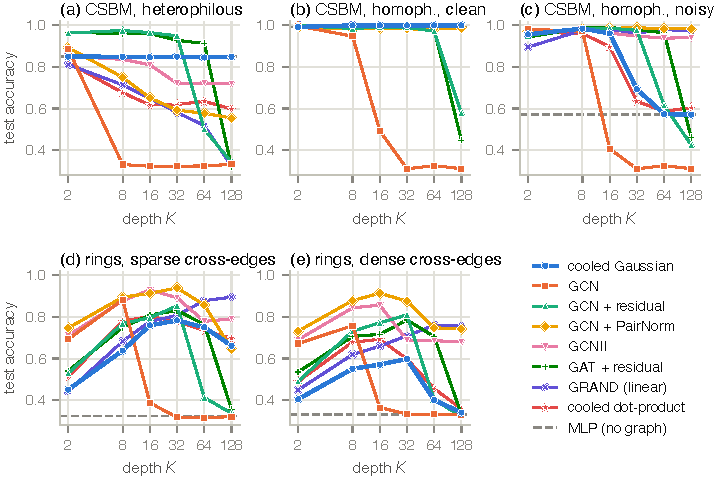
\includegraphics[width=\linewidth]{figures/fig6_depth_synthetic.pdf}
\caption{\textbf{Trained networks against depth} on the synthetic tasks (E6b, E7): mean test accuracy over 5 seeds, each run tuned over 8
configurations. (a--c)~CSBMs with 3 classes; (d--e)~ring task in which $2\%$ of the nodes carry the class. Dashed: MLP. All 13 models with
confidence intervals are in \cref{tab:train-e6b,tab:train-e7}; stars: the cooled dot-product network of \cref{sec:learned}. Gaussian attention with constant temperature is within $0.007$ of the
cooled version on the CSBMs and up to $0.10$ better on the rings at depth $K\ge32$.}
\label{fig:depth-synthetic}
\end{figure}

The theory describes the untrained dynamics~\eqref{eq:model}. We now train it. Our Gaussian networks map the input to $z=Wx$ with a linear
layer, apply $K$ parameter-free layers of~\eqref{eq:model}, and classify the final states with a linear readout. By \cref{rem:metric}, $W$
is a learned metric. The scale $c$ of the cooled temperature $c/\log(l+11)$, or a constant temperature $T$, is learned too. It is
initialised at $m$ times the median squared edge length, with $m\in\{1,1/30\}$ chosen on validation data. We compare with an MLP,
GCN~\citep{kipf2017}, residual GCN, GCN with PairNorm~\citep{zhao2020pairnorm}, GCNII~\citep{chen2020gcnii}, APPNP~\citep{klicpera2019},
SGC~\citep{wu2019sgc}, GAT~\citep{velickovic2018}, residual GAT and linear GRAND~\citep{chamberlain2021}. Each (task, model, depth, seed)
picks the best of 8 configurations on validation accuracy: learning rate, dropout and one model-specific hyperparameter
(\cref{app:exp}).

\paragraph{Synthetic tasks (E6b, E7).} We use three contextual SBMs~\citep{deshpande2018} with 3 classes of 150 nodes: homophilous with
clean features, homophilous with noisy features, and heterophilous. We also use a long-range task: three rings of 200 nodes with random
cross-class edges, where only $2\%$ of the nodes carry class information and a typical node is 12 hops from the nearest informative one.
\Cref{fig:depth-synthetic} shows test accuracy against depth $K\in\{2,\dots,128\}$. GCN, SGC and GAT fall to chance by $K=16$--$32$ on
every task. Residual connections postpone the collapse to $K=64$--$128$.

The Gaussian networks behave differently in a way the theory explains. By \cref{prop:dichotomy}, a deep network of this kind ends in a
partition of the nodes into clusters, and training chooses the partition through $W$ and $c$. Two partitions are always available.
One cluster per connected component is oversmoothing. The partition into singletons, the frozen phase, reproduces the MLP. Which phase a
run reaches is set mostly by the initial temperature.
\begin{itemize}
\item In the heterophilous CSBM, validation picks the cold start $m=1/30$ in all 30 runs (6 depths, 5 seeds) of each Gaussian model. The
network then matches the MLP seed by seed, within $0.015$ in test accuracy. At $K=128$ the Gaussian networks are the only models at the MLP level of
$0.85$. Every baseline is at least $0.12$ below it.
\item In the clean homophilous CSBM, the default start reaches the class partition and keeps it. The cooled network has accuracy $0.999$
at every depth from 8 to 128, the best or within $0.001$ of the best.
\item In the noisy homophilous CSBM the class partition is not reachable at depth. The default start gives $0.984$ at $K=8$, within
$0.003$ of the best model. From $K=64$ on it collapses to chance ($0.33$, effective rank $1.5$--$3$), and the cold start freezes at the MLP
level ($0.57$). At $K=32$ two of five seeds still reach the class partition.
\end{itemize}
The noisy regime is the case in which the design rule of \cref{sec:prediction} cannot be met. Class means are $1.5$ apart and the noise
has standard deviation $1$ in every coordinate. Along any direction, a large share of the within-class edges is about as long as the
distance between class means, so no metric separates the two scales by the factor $\kappa$ that the rule needs. A shallow network stops before the limit and can still smooth partially. A deep one cannot.

On the ring task the Gaussian networks improve with depth up to $K=32$, but stay well below PairNorm and GCNII. The cooled network peaks
at $0.60$ (dense cross-edges) and $0.78$ (sparse), against $0.91$ and $0.94$ for PairNorm. Similarity-based attention has nothing to work
with at nodes whose features are pure noise. Here the constant temperature is better at depth, by up to $0.10$, consistent with cooling
sharpening the attention and so shortening the range of propagation.

\paragraph{Cooled dot-product attention.} The same network with the learned score $\langle W_Qz_i,W_Kz_j\rangle$ of \cref{sec:learned}
($J=W_Q^\top W_K$, shared by all layers) behaves like the Gaussian one where a coarse partition is wanted. It reaches $0.995$--$0.998$ at every depth on
the clean CSBM, and on the rings it peaks higher, at $0.80$ (sparse) and $0.69$ (dense) for $K=16$, but still below PairNorm. The difference is the
frozen phase. A dot-product score need not be largest at $j=i$, so some margins can be negative, and then no temperature makes every node
keep its own state (\cref{prop:margin}). On the heterophilous CSBM, validation picks the cold start in 28 of 30 runs and the
network still falls from $0.82$ at $K=2$ to $0.60$--$0.68$ for $K\ge8$, against $0.85$ for the MLP and the Gaussian networks. On the noisy
CSBM it holds $0.96$ to $K=8$ and drops to about $0.6$ from $K=32$ on.

\paragraph{Do trained networks reach the predicted partition?} For each of the 150 reported dot-product runs we rerun the network's own dynamics,
with its learned $J$ and $c$, for 4000 layers from its input states (\cref{app:exp}); at layer $K$ this reproduces the trained network's test
accuracy to $3\cdot10^{-8}$. The two starts then behave differently.
\begin{itemize}
\item The 46 cold-start runs are close to their limit at depth $K$. Run to 4000 layers they lose $0.004$ test accuracy on average (at most
$0.048$), and every one settles into a partition with a few to several hundred clusters. The directed rule applied after $t_1=20$ layers
recovers it with mean ARI $0.97$, below $0.9$ in 2 runs, and the symmetric rule gets $0.96$. Applied at $t_1=0$ both fail (ARI $0.13$
and $0.00$). In trained networks the rule thus needs a few layers before it applies, as in E9, and five are not enough (ARI $0.66$).
\item The 104 default-start runs rely on the transient. Run to 4000 layers they lose $0.29$ test accuracy on average and up to $0.70$. In
47 of them, all on the rings or the clean CSBM, the partition is still changing at layer 4000. In the 57 others the final partition has one to
a few clusters, and the directed rule at $t_1=20$ gets mean ARI $0.88$ (symmetric rule $0.94$). Its errors are again one-sided: in 56 of the
57 runs no edge that it predicts to persist ends merged, and most misses are runs in which it predicts fewer clusters than form, often one where two form.
\end{itemize}
Training makes $J_s$ indefinite in 37 runs, 31 of them on the rings, with $\lambda_{\min}(J_s)$ down to $-1.8$. None of them oscillates: the
largest change in the last layer is $4\cdot10^{-5}$. \Cref{prop:oscillation} is for a specific configuration, and trained networks do not
reach one. A trained network at depth $K$ is thus either near its limiting partition, which the directed rule predicts after a few
layers, or in a transient whose accuracy the limit does not keep.

\paragraph{Real graphs (E8).} We train the Gaussian networks and the ten baselines on Roman-empire and Amazon-ratings with $K\in\{2,4,8,16,32\}$ and width 64, on
three of the ten official splits, with the learning rate tuned per model and depth on split 0 (\cref{tab:train-e8}). Roman-empire repeats
the heterophilous CSBM. The cooled network freezes, ending with $21{,}500$--$22{,}200$ clusters on $22{,}662$ nodes, and holds the MLP
accuracy ($0.642$--$0.643$ against $0.644$) at every depth, while GCN, SGC and GAT fall to $0.13$--$0.19$ by $K=32$. Residual GCN and residual
GAT are much better at moderate depth ($0.79$--$0.80$ at $K=4$--$8$) but drop to $0.60$--$0.63$ at $K=32$. On Amazon-ratings the cooled
network ($0.415$--$0.419$ for $K\le16$) beats the MLP ($0.386$) but not PairNorm ($0.470$).

Run to 4000 layers, the trained cooled Gaussian networks fall into the same two groups as the dot-product networks. On Roman-empire their test
accuracy changes by at most $0.006$, and the threshold-graph rule applied after $K$ layers recovers the final partition with ARI
$0.79$--$0.99$. On Amazon-ratings every network falls to the majority-class level ($0.37$--$0.38$), and its partition is still changing at
layer 4000 (ARI between layers 2000 and 4000 as low as $0.12$): these networks use the transient.
On Peptides-func, a long-range molecular benchmark, propagation helps (\cref{tab:train-e8-pep}, one seed, $K\in\{2,8,32\}$). Residual GAT
reaches average precision $0.421$ at $K=8$ against $0.253$ for the MLP, and plain GCN falls from $0.349$ at $K=2$ to $0.169$ at $K=32$,
below the MLP. Both Gaussian networks stay at the MLP level ($0.246$--$0.254$) at every depth, cooled or not: on these graphs they keep the
MLP's accuracy but do not use the graph.

\paragraph{Summary.} The cooled Gaussian network is an analysable model, not a competitive architecture. Because the frozen phase is always
reachable, its mean accuracy is never more than $0.005$ below the MLP's at any depth on the seven node tasks, and its average precision on
Peptides-func never more than $0.007$ below; residual and normalised baselines beat
it wherever propagation helps. What the theory adds is prediction: which distinctions survive, which metric keeps them, and whether the
accuracy of a trained network at depth $K$ is a property of its limit or of a transient.

%=====================================================================
\section{Discussion and limitations}\label{sec:discussion}
%=====================================================================

\paragraph{What is proved and what is not.} \Cref{thm:two-block,thm:chain,thm:rescue,thm:planted} and
\cref{prop:dichotomy,prop:sharp,prop:third} and \cref{cor:topology} are analytic. So are \cref{thm:learned,prop:margin,prop:oscillation,prop:separation}. \Cref{thm:cap} is computer-assisted. The survival of
noisy blocks with diameter above $\sqrt c$ (E4) is an observation without proof, and so is the dependence of the critical weaker margin
on the partner margin in \cref{fig:learned}(a), which is a float computation. The scaling limit
in \cref{thm:rescue}(c) holds beyond an explicit but astronomically large $t_0$ near the corner $x=2/3$. The quantitative chain theory is
for scalar, layer-constant features; \cref{prop:dichotomy,thm:planted} cover vector features on general graphs, but only through
sufficient conditions.

\paragraph{Model scope.} \Cref{eq:model} has no value matrix, nonlinearity, residual connection or multiple heads. \Cref{rem:metric} covers
a fixed learned metric and \cref{sec:learned} a fixed quadratic query--key score. A layer-dependent score changes the margins layer by layer,
and our rules then apply only between changes. For learned scores the exact theory is for two blocks; on general graphs we have only the
separation result of \cref{prop:separation}, and whether \cref{prop:dichotomy} extends to scores with $J_s\succ0$ is open. Logarithmic cooling is a modelling choice that makes the threshold finite and nontrivial. We do not claim that it is the best
schedule for training.

\paragraph{Using the theory.} The early-depth rule is a cheap diagnostic for distance-based and query--key attention: run a few layers,
threshold the directed margins at $\kappa(t_0+t_1)^2$, and read off the partition the network converges to. Comparing it with the labels shows
which distinctions depth will erase, and the design rule says how to scale a metric so that it keeps the right ones. In trained networks the
same comparison tells whether accuracy at the trained depth will survive further depth. Extending the theory to layer-dependent scores, value
maps and residual connections is the main open step.

\bibliographystyle{plainnat}
\bibliography{references}

\clearpage
\appendix
% Appendix of main.tex (input after \appendix).

%=====================================================================
\section{Proofs for Sections~\ref{sec:setup} and~\ref{sec:twoblock}}\label{app:twoblock}
%=====================================================================

\begin{proof}[Proof of \cref{prop:constT}]
Each $h_i(t+1)$ is a convex combination of $\{h_j(t)\}$, so the feature diameter $R_t$ is nonincreasing and
$\alpha_{ij}(t)\ge e^{-\|W\|^2R_0^2/T}/\Nmax=:\gamma>0$ on every edge, including self-loops. A product of stochastic matrices whose
positive entries are bounded below by $\gamma$ on a fixed connected graph with self-loops is a consensus product, at an exponential
rate~\citep{moreau2005}. Indeed, every product of $\diam(G)$ consecutive matrices has a column bounded below by $\gamma^{\diam(G)}$, so its
Dobrushin coefficient is at most $1-\gamma^{\diam(G)}$.
\end{proof}

\begin{proof}[Proof of \cref{lem:reduction}]
Let $z_A,z_B$ be the block values and $a=s_t^{-d^2}$. A node of $A$ sees $k_A$ nodes at distance $0$ and $e_A$ nodes at distance $d$, so
$z_A'=(k_Az_A+e_Aa\,z_B)/(k_A+e_Aa)=z_A+\frac{\rho_Aa}{1+\rho_Aa}(z_B-z_A)$, and symmetrically for $B$. All nodes of a block receive the same
update, so the features stay block-constant, and
\[
z_B'-z_A'=(z_B-z_A)\Big(1-\frac{\rho_Aa}{1+\rho_Aa}-\frac{\rho_Ba}{1+\rho_Ba}\Big)=(z_B-z_A)\,\frac{1-Pa^2}{(1+\rho_Aa)(1+\rho_Ba)} .\qedhere
\]
\end{proof}

\paragraph{Properties of $F_t$.} For $a\in[0,1)$ we have $0<\psi(a)\le\frac{1-Pa^2}{1+\lambda a+Pa^2}\le\frac1{1+\lambda a}\le1$, because
$P\le1$. The function $\psi$ is decreasing in $a$ and nonincreasing in $\rho_A$ and $\rho_B$. Since $a=s_t^{-d^2}$ decreases in $d$,
$F_t'(d)=\psi(a)+d\,\psi'(a)\,\partial_da>0$. So $F_t$ is a continuous increasing bijection of $(0,\infty)$ with $F_t(d)\le d$. For fixed $d$
and $t$, $F_t(d)$ is nondecreasing in $t_0$ and nonincreasing in $\rho_A,\rho_B$. Write $\Phi_k=F_{k-1}\circ\dots\circ F_0$, so that
$d_k=\Phi_k(d_0)$, and note that the trajectory from $d_0$ at offset $t_0$ continues after $k$ steps as the trajectory from $\Phi_k(d_0)$
at offset $t_0+k$.

\paragraph{Certificate C1 (\cref{thm:two-block}(vi), second half).} Suppose $d_u\ge\delta$ for all $u<t$. Then $a_u\le s_u^{-\delta^2}\le q$,
and
\[
-\log\psi(a)=\log(1+\rho_Aa)+\log(1+\rho_Ba)-\log(1-Pa^2)\le\lambda a+\frac{Pa^2}{1-Pa^2}\le\Lambda_\delta\,a .
\]
With $\sum_{u\ge0}(t_0+u)^{-\delta^2}\le\int_{t_0-1}^\infty x^{-\delta^2}dx=\frac{(t_0-1)^{1-\delta^2}}{\delta^2-1}$ we get
$\log d_t\ge\log d_0-\Lambda_\delta\frac{(t_0-1)^{1-\delta^2}}{\delta^2-1}\ge\log\delta$, and induction on $t$ closes the argument.

\begin{proof}[Proof of \cref{thm:two-block}]
\emph{(i)} The sequence $d_t$ is positive and nonincreasing, so it converges. If $d_T\le1$, then $d_t\le1$ and $a_t\ge s_t^{-1}$ for all
$t\ge T$. Hence $d_{t+1}\le d_t/(1+\lambda a_t)\le d_t\exp(-\frac{\lambda}{1+\lambda}s_t^{-1})$, and $\sum_ts_t^{-1}=\infty$ gives $d_t\to0$.
Otherwise $d_t>1$ for all $t$ and $d_\infty\ge1$.

\emph{(ii)} By (i), the merge set is $M(t_0)=\bigcup_T\{d_0:\Phi_T(d_0)\le1\}$. If $\Phi_T(d_0)=1$ then $\Phi_{T+1}(d_0)<1$, so
$M(t_0)=\bigcup_T\Phi_T^{-1}((0,1))=\bigcup_T(0,\Phi_T^{-1}(1))$, an open interval $(0,\kappa)$. Since $F_0(1)<1$, $1\in M(t_0)$ and
$\kappa>1$. Finiteness follows from (vi). Since $\kappa\notin M(t_0)$, the threshold gap itself persists.

\emph{(iii)} $d_\infty(d_0)=\inf_T\Phi_T(d_0)$ is nondecreasing and, as an infimum of continuous functions, upper semicontinuous. A
nondecreasing upper semicontinuous function is right-continuous. Since $\kappa$ persists, $d_\infty(\kappa)\ge1$. Suppose
$d_\infty(\kappa)=1+2\eta$ with $\eta>0$, and let $\delta=1+\eta/2$. Because $(t_0+T-1)^{1-\delta^2}\to0$, there is $T$ such that \eqref{eq:C1}
holds at offset $t_0+T$ for every initial value $\ge1+\eta$. Since $\Phi_T(\kappa)\ge1+2\eta$ and $\Phi_T$ is continuous, some $d_0<\kappa$
has $\Phi_T(d_0)\ge1+\eta$. By C1 at offset $t_0+T$, the trajectory from $d_0$ stays above $\delta>1$, so $d_0$ persists. This contradicts
$d_0\in M(t_0)=(0,\kappa)$, so $d_\infty(\kappa)=1$.

\emph{(iv)} $M(t_0+k)=\Phi_k(M(t_0))=(0,\Phi_k(\kappa(t_0)))$, because $\Phi_k$ is an increasing bijection. For monotonicity, let
$t_0\le t_0'$ (or $\rho\ge\rho'$ componentwise) and compare the trajectories $d_t,d_t'$ from the same $d_0$:
$d'_{t+1}=F'_t(d'_t)\ge F'_t(d_t)\ge F_t(d_t)=d_{t+1}$. Hence $M(t_0')\subseteq M(t_0)$ (respectively $M(\rho')\subseteq M(\rho)$).

\emph{(vi), lower bound.} Let $d_0=1+\varepsilon$ persist, for instance $\varepsilon=\kappa-1$. Then $1\le d_\infty\le d_t\le d_0$, so
$s_t^{-1}\ge a_t\ge s_t^{-(1+\varepsilon)^2}$. Using $\log(1+y)\ge y/(1+y)$ and $a_t\le1/t_0$,
\begin{align*}
\log(1+\varepsilon)\ &\ge\ \log\frac{d_0}{d_\infty}=\sum_t-\log\psi(a_t)\ \ge\ \sum_t\big[\log(1+\rho_Aa_t)+\log(1+\rho_Ba_t)\big]\\
&\ge\ \lambda_-\sum_{t\ge0}s_t^{-(1+\varepsilon)^2}\ \ge\ \lambda_-\,\frac{t_0^{-y}}{y},
\end{align*}
with $y=2\varepsilon+\varepsilon^2$. Since $\log(1+\varepsilon)\le\varepsilon$, we get $\varepsilon(2\varepsilon+\varepsilon^2)\ge\lambda_-t_0^{-(2\varepsilon+\varepsilon^2)}$. The left
side increases and the right side decreases in $\varepsilon$, so $\varepsilon\ge\varepsilon_-$.

Part (v) is proved below.
\end{proof}

\subsection{Proof of \cref{thm:two-block}(v): barriers}\label{app:second}

Write $\tau_t=\log s_t$ and $\Delta_t=\tau_{t+1}-\tau_t=\log(1+e^{-\tau_t})\in\big[e^{-\tau_t}(1-\tfrac12e^{-\tau_t}),\,e^{-\tau_t}\big]$. Let
$c(\tau)=c_0+(\beta\log\log\tau+k)/\log\tau$ with constants $c_0,\beta,k$ (the proof of (v) uses $\beta=k=0$, that of \cref{prop:third}
uses $\beta=\frac14$), and for $\tau>e$ let
\[
N_c(\tau)=\log\tau-\tfrac12\log\log\tau+c(\tau),\qquad X_c(\tau)=N_c(\tau)/\tau,\qquad\text{so}\qquad
e^{-2\tau X_c(\tau)}=e^{-2c(\tau)}\,\frac{\log\tau}{\tau^2}. \tag{$*$}
\]

\begin{lemma}[barrier functions]\label{lem:barrier}
There is $\tau_1$ such that on $[\tau_1,\infty)$: $0<X_c\le1$, $X_c'<0<X_c''$, $\tau X_c^2\le1$, and
\[
\frac{\tau^2|X_c'(\tau)|}{\log\tau}=1-r_c(\tau),\qquad r_c(\tau)=\frac{\frac12\log\log\tau-c(\tau)+1-\frac1{2\log\tau}+\tau c'(\tau)}{\log\tau},
\]
where $r_c(\tau)\to0$ and $\tau c'(\tau)=O(\log\log\tau/(\log\tau)^2)$. Moreover $\tau X_c(\tau)^2\to0$ and $r_c(\tau+\Delta)=r_c(\tau)+O(e^{-\tau})$ for $0\le\Delta\le e^{-\tau}$.
\end{lemma}
\begin{proof}
With $u=\log\tau$, $\tau c'=(\beta-\beta\log u-k)/u^2$. Then $N_c'=(1-\frac1{2\log\tau})/\tau+c'$, so
$\tau^2X_c'=\tau N_c'-N_c=-(N_c-1+\frac1{2\log\tau}-\tau c')$, which gives the formula for $r_c$ and $X_c'<0$ for large $\tau$. Further
$\tau^3X_c''=2N_c-2\tau N_c'+\tau^2N_c''=2\log\tau+O(\log\log\tau)>0$, $\tau X_c^2=N_c^2/\tau\to0$, and $r_c'(\tau)=O(1/\tau)$.
\end{proof}

For $0\le a\le e^{-\tau}$ and $\tau\ge1$ we use two bounds on $\psi$. Since $\psi(a)\ge(1-Pa^2)(1-\lambda a-Pa^2)\ge1-\lambda a-2Pa^2$ and $P\le1$,
\begin{equation}\label{eq:P1}
1-\psi(a)\le a\,(\lambda+2e^{-\tau}).
\end{equation}
Since $1-\psi(a)=\frac{\lambda a+2Pa^2}{1+\lambda a+Pa^2}\ge\frac{\lambda a}{1+(\lambda+1)a}$,
\begin{equation}\label{eq:P2}
1-\psi(a)\ge\lambda a\,\big(1-(\lambda+1)e^{-\tau}\big).
\end{equation}

\begin{proof}[Proof of \cref{thm:two-block}(v)]
Let $L=\log t_0$ and fix $\eta>0$.

\emph{Upper bound.} Let $X=X_c$ with $c\equiv\frac12\log\lambda+\eta$. We claim that there is $\tau_2\ge\tau_1$ with
\begin{equation}\label{eq:barrier-up}
F_t\big(1+X(\tau_t)\big)\ \ge\ 1+X(\tau_{t+1})\qquad\text{whenever }\tau_t\ge\tau_2 .
\end{equation}
Write $\tau=\tau_t$, $\Delta=\Delta_t$ and $d=1+X(\tau)$. Then $a=s_t^{-d^2}=e^{-\tau}e^{-2\tau X}e^{-\tau X^2}\le e^{-\tau}\lambda^{-1}e^{-2\eta}\log\tau/\tau^2$ by
($*$), and \eqref{eq:P1} gives
\[
d-F_t(d)=d\,(1-\psi(a))\ \le\ e^{-\tau}\,(1+X)\Big(1+\frac{2e^{-\tau}}{\lambda}\Big)\,e^{-2\eta}\,\frac{\log\tau}{\tau^2}.
\]
By convexity, $X(\tau)-X(\tau+\Delta)\ge\Delta\,|X'(\tau+\Delta)|\ge e^{-\tau}(1-\frac12e^{-\tau})|X'(\tau+\Delta)|$, and by \cref{lem:barrier}
$|X'(\tau+\Delta)|=(1+o(1))\log\tau/\tau^2$ as $\tau\to\infty$, uniformly in $\Delta\in[0,e^{-\tau}]$. Since $e^{-2\eta}<1$ and
$(1+X)(1+2e^{-\tau}/\lambda)\to1$, we get $X(\tau)-X(\tau+\Delta)\ge d-F_t(d)$ for large $\tau$, which is \eqref{eq:barrier-up}.
Now let $L\ge\tau_2$ and $d_0\ge1+X(L)$. Since $F_t$ is increasing, induction with \eqref{eq:barrier-up} gives
$d_{t+1}=F_t(d_t)\ge F_t(1+X(\tau_t))\ge1+X(\tau_{t+1})>1$ for all $t$. By (i) the gap persists. Hence
$\kappa(t_0)\le1+X_{\frac12\log\lambda+\eta}(L)$ for all large $t_0$.

\emph{Lower bound.} Let $Y=X_c$ with $c\equiv\frac12\log\lambda-\eta$. We claim that there is $\tau_3\ge\tau_1$ with
\begin{equation}\label{eq:barrier-down}
F_t\big(1+Y(\tau_t)\big)\ \le\ 1+Y(\tau_{t+1})\qquad\text{whenever }\tau_t\ge\tau_3 .
\end{equation}
With $d=1+Y(\tau)$ we have $a=e^{-\tau}\lambda^{-1}e^{2\eta}e^{-\tau Y^2}\log\tau/\tau^2\le e^{-\tau}$ for large $\tau$, and \eqref{eq:P2} gives
\[
d-F_t(d)\ \ge\ e^{-\tau}\,(1+Y)\,e^{2\eta}\,e^{-\tau Y^2}\big(1-(\lambda+1)e^{-\tau}\big)\frac{\log\tau}{\tau^2},
\]
while convexity gives $Y(\tau)-Y(\tau+\Delta)\le\Delta|Y'(\tau)|\le e^{-\tau}(1-r_c(\tau))\log\tau/\tau^2$. Since $e^{2\eta}>1$ and $\tau Y^2\to0$, this
proves \eqref{eq:barrier-down} for large $\tau$. Now let $L\ge\tau_3$ and $d_0=1+Y(L)$. By induction, $d_t\le1+Y(\tau_t)$ for all $t$. Suppose
the gap persists. By (i), $d_t>1$ for all $t$, so $s_t^{-(1+Y(\tau_t))^2}\le a_t\le e^{-\tau_t}$. By \eqref{eq:P2} and ($*$),
\[
d_t-d_{t+1}=d_t(1-\psi(a_t))\ \ge\ \lambda a_t\big(1-(\lambda+1)e^{-\tau_t}\big)\ \ge\ e^{2\eta}\big(1-\epsilon(\tau_t)\big)\,g(s_t),
\qquad g(s)=\frac{\log\log s}{s\,(\log s)^2},
\]
with $\epsilon(\tau)=1-e^{-\tau Y(\tau)^2}(1-(\lambda+1)e^{-\tau})\to0$. Choose $\tau_4\ge\tau_3$ such that $1-\epsilon(\tau)\ge e^{-\eta}$ and $g$ is
decreasing for $\log s\ge\tau_4$, and let $L\ge\tau_4$. Summing over $t$ and substituting $\tau=\log s$,
\begin{align*}
d_0-1&\ \ge\ \sum_{t\ge0}(d_t-d_{t+1})\ \ge\ e^{\eta}\sum_{t\ge0}g(t_0+t)\ \ge\ e^{\eta}\int_{t_0}^\infty g(s)\,ds\\
&\ =\ e^{\eta}\int_L^\infty\frac{\log\tau}{\tau^2}\,d\tau\ =\ e^{\eta}\,\frac{\log L+1}{L}.
\end{align*}
But $d_0-1=Y(L)=(\log L-\frac12\log\log L+\frac12\log\lambda-\eta)/L$, which is smaller than $e^\eta(\log L+1)/L$ for large $L$. This is a
contradiction, so $d_0=1+Y(L)$ merges, and $\kappa(t_0)>1+X_{\frac12\log\lambda-\eta}(L)$ for all large $t_0$.

Since $\eta>0$ was arbitrary, $(\kappa-1)L-(\log L-\frac12\log\log L+\frac12\log\lambda)\to0$. In physical units
$d_{\rm crit}^2=c\kappa^2=c+2c(\kappa-1)+c(\kappa-1)^2$, where $c/L=T_0$, $\log L=\log(c/T_0)$ and $c(\kappa-1)^2=T_0\,O((\log L)^2/L)=o(T_0)$.
\end{proof}

\begin{proof}[Proof of \cref{cor:topology}]
Subtract the expansions of (v) for $(\rho_A,\rho_B)$ and $(\rho_A',\rho_B')$; in physical units multiply by $2c\kappa$, using
$c/\log t_0=T_0$ and $\kappa\to1$.
\end{proof}

\begin{remark}[where the third term comes from]\label{rem:third-heuristic}
In the continuum limit $dx/d\tau=-\lambda e^{-2\tau x}$ (dropping terms of relative order $x$ and $e^{-\tau}$), write
$x=(N_{\frac12\log\lambda}(\tau)+y/2)/\tau$. Then
\[
\frac{\tau y'}{2}=\log\tau\,(1-e^{-y})-\tfrac12\log\log\tau+\tfrac12\log\lambda-1+\frac y2+\frac1{2\log\tau}.
\]
The linearisation $\tau\,\delta y'\approx2\log\tau\,\delta y$ shows that the critical solution is repelling, so it stays near the zero of the right
side, $y^*=(\log\log\tau-\log\lambda+2)/(2\log\tau)+O\big((\log\log\tau)^2/(\log\tau)^2\big)$. This is the third term of \cref{prop:third};
the barrier proof below makes it rigorous for the discrete map.
\end{remark}

\begin{proof}[Proof of \cref{prop:third}]
Fix $\eta>0$, let $\delta_\pm(\tau)=(\log\log\tau-\log\lambda+2\pm\eta)/(4\log\tau)$ and $c_\pm=\frac12\log\lambda+\delta_\pm$, and let
$X=X_{c_+}$ and $Y=X_{c_-}$. Since $\delta_\pm=O(\log\log\tau/\log\tau)$, \cref{lem:barrier} gives
\begin{align*}
1-r_{c_\pm}(\tau)&=1-\frac{\frac12\log\log\tau-\frac12\log\lambda+1}{\log\tau}+O\Big(\frac{\log\log\tau}{(\log\tau)^2}\Big),\\
e^{-2\delta_\pm(\tau)}&=1-\frac{\frac12\log\log\tau-\frac12\log\lambda+1\pm\frac\eta2}{\log\tau}+O\Big(\frac{(\log\log\tau)^2}{(\log\tau)^2}\Big),
\end{align*}
so that
\begin{equation}\label{eq:third-key}
\big(1-r_{c_\pm}(\tau)\big)-e^{-2\delta_\pm(\tau)}=\pm\frac{\eta}{2\log\tau}+O\Big(\frac{(\log\log\tau)^2}{(\log\tau)^2}\Big).
\end{equation}
We repeat the proof of (v), with $e^{\mp2\eta}$ replaced by $e^{-2\delta_\pm(\tau)}$ in the bounds on $a$.

\emph{Upper bound.} As there, \eqref{eq:barrier-up} holds if
\[
\big(1-\tfrac12e^{-\tau}\big)\big(1-r_{c_+}(\tau+\Delta)\big)\frac{\log(\tau+\Delta)}{(\tau+\Delta)^2}\ \ge\
(1+X)\Big(1+\frac{2e^{-\tau}}{\lambda}\Big)e^{-2\delta_+(\tau)}\frac{\log\tau}{\tau^2}.
\]
By \cref{lem:barrier}, every factor other than $1-r_{c_+}(\tau)$ and $e^{-2\delta_+(\tau)}$ is $1+O(\log\tau/\tau)$, so this follows from
\eqref{eq:third-key} for large $\tau$. Hence $\kappa(t_0)\le1+X(L)$ for large $t_0$.

\emph{Lower bound.} As there, \eqref{eq:barrier-down} holds if
$(1+Y)\,e^{-2\delta_-(\tau)}e^{-\tau Y^2}(1-(\lambda+1)e^{-\tau})\ge1-r_{c_-}(\tau)$, which follows from \eqref{eq:third-key} in the same way.
Let $d_0=1+Y(L)$, so that $d_t\le1+Y(\tau_t)$ for all $t$ by induction, and suppose that the gap persists. Then
$d_t-d_{t+1}\ge e^{-2\delta_-(\tau_t)}(1-\epsilon(\tau_t))\,g(s_t)$ with $\epsilon(\tau)\le\tau Y(\tau)^2+(\lambda+1)e^{-\tau}=O((\log\tau)^2/\tau)$.
For large $\tau$, $\delta_-$ is decreasing, so with $\bar\epsilon(L)=\sup_{\tau\ge L}\epsilon(\tau)$,
\begin{align*}
L\,(d_0-1)&\ \ge\ e^{-2\delta_-(L)}\big(1-\bar\epsilon(L)\big)(\log L+1)\ \ge\ \log L+1-2\delta_-(L)\log L-O\Big(\frac{\log\log L}{\log L}\Big)\\
&\ =\ \log L-\tfrac12\log\log L+\tfrac12\log\lambda+\frac\eta2-o(1),
\end{align*}
using $e^{-x}\ge1-x$. But $L(d_0-1)=LY(L)=\log L-\frac12\log\log L+\frac12\log\lambda+\delta_-(L)$ and $\delta_-(L)\to0$, a contradiction for
large $L$. Hence $\kappa(t_0)>1+Y(L)$.

Since $\eta>0$ was arbitrary, $(\kappa-1)L=\log L-\frac12\log\log L+\frac12\log\lambda+\frac{\log\log L-\log\lambda+2+o(1)}{4\log L}$. For the
topology shift, subtract the expansions for $\lambda$ and $\lambda'$: the third terms differ by $-\log(\lambda/\lambda')/(4\log L)$.
\end{proof}

%=====================================================================
\section{Proofs for chains}\label{app:chains}
%=====================================================================

\paragraph{Derivation of \eqref{eq:chain}.} By symmetry, layer-constant features stay layer-constant. A node of layer $l$ sees $m$ nodes
of layers $l-1$, $l$, $l+1$ with weights $w_{l-1},1,w_l$, so $x_l'=(w_{l-1}x_{l-1}+x_l+w_lx_{l+1})/D_l$. Then
$x_l'-x_l=(w_lg_l-w_{l-1}g_{l-1})/D_l$, and $g_l'=x_{l+1}'-x_l'$ equals
$g_l\big(1-\frac{w_l}{D_l}-\frac{w_l}{D_{l+1}}\big)+\frac{w_{l+1}g_{l+1}}{D_{l+1}}+\frac{w_{l-1}g_{l-1}}{D_l}$. With $D_l=A+w_l$ and
$D_{l+1}=B+w_l$, the bracket equals $(AB-w_l^2)/(D_lD_{l+1})$.

\begin{proof}[Proof of \cref{lem:comparison}]
All terms of \eqref{eq:chain} are nonnegative, since $AB\ge1\ge w_l^2$. It remains to show $(AB-w^2)(1+w)\ge(1-w)(A+w)(B+w)$ for $A,B\ge1$ and
$w\in[0,1]$; the difference equals $w\,[(A-1)B+A(B-1)+w(A+B-2)]\ge0$. Dropping the push terms gives
$g_l'\ge g_l\frac{1-w_l}{1+w_l}=F_t(g_l)$.
\end{proof}

\begin{proof}[Proof of \cref{thm:chain}]
(a) By \cref{lem:comparison} and the monotonicity of $F_t$, induction gives $g_l(t_1+k)\ge d_k$, where $d$ is the isolated trajectory at offset
$t_0+t_1$ from $\kappa(t_0+t_1)$. By \cref{thm:two-block}(ii),(iii), $d_k>1$ for all $k$.
(b) is (a) with $t_1=0$.
(c) One-sidedness is (a). If $g_l(t_1)\ge\kappa(t_0+t_1)$, then by \cref{lem:comparison} and \cref{thm:two-block}(iv),
$g_l(t_1+1)\ge F_{t_1}(g_l(t_1))\ge F_{t_1}(\kappa(t_0+t_1))=\kappa(t_0+t_1+1)$, where $F_{t_1}$ is taken at offset $t_0$. So the declared set
is nondecreasing. A merging gap has $g_l(t_1)\to0<1<\kappa(t_0+t_1)$ and is always declared merging. A persisting gap with $g_l(t)\to g_\infty>1$
is eventually declared persisting, because $\kappa(t_0+t_1)\to1$ by \cref{thm:two-block}(v).
\end{proof}

\subsection{Three layers}\label{app:three}

Let $u=x_2-x_1$, $v=x_3-x_2$, $w_1=s_t^{-u^2}$, $w_2=s_t^{-v^2}$, $D_1=1+w_1$, $D_2=1+w_1+w_2$, $D_3=1+w_2$. Write $D:=u+v$,
$h:=u+v/2$ and $\tilde h:=v+u/2$. By \cref{prop:dichotomy}, the limits $u_\infty,v_\infty$ exist and lie in $\{0\}\cup[1,\infty)$. Define
\begin{align*}
U_+(v_0;t_0)&:=\inf\{u:\ \text{gap 1 persists from }(u',v_0)\ \forall u'\ge u\},\\
U_-(v_0;t_0)&:=\sup\{u:\ \text{gap 1 merges from }(u',v_0)\ \forall u'\le u\},
\end{align*}
so that $U_-\le U_+$ and $u^*\in[U_-,U_+]$.

\begin{lemma}[identities]\label{lem:id}
With $F_t$ the isolated map,
\begin{align}
u'&=F_t(u)+\frac{w_2}{D_2}\Big(v+\frac{w_1u}{D_1}\Big), &
v'&=F_t(v)+\frac{w_1}{D_2}\Big(u+\frac{w_2v}{D_3}\Big),\label{eq:I1}\\
h'&=h-w_1\Big[u\Big(\frac1{2D_2}+\frac1{D_1}\Big)+\frac{w_2v}{2D_2D_3}\Big], &
\tilde h'&=\tilde h-w_2\Big[v\Big(\frac1{2D_2}+\frac1{D_3}\Big)+\frac{w_1u}{2D_1D_2}\Big],\label{eq:I2}\\
D'&=D-\frac{w_1u}{D_1}-\frac{w_2v}{D_3}. \label{eq:I3}
\end{align}
Consequently $h,\tilde h,D$ are nonincreasing, $u\le h$, $v\le\tilde h$, $u,v\le D\le D_0$, and
\begin{align}
&(1-2w_1)u\le u'\le(1-w_1)u+w_2(u+v),\qquad (1-2w_2)v\le v'\le(1-w_2)v+w_1(u+v),\label{eq:bounds}\\
&0\le h-h'\le\tfrac32\,w_1(u+v). \label{eq:hloss}
\end{align}
\end{lemma}
\begin{proof}
Put $x_1=0$, $x_2=u$, $x_3=u+v$. Then $x_1'=w_1u/D_1$ and $x_2'=(u(1+w_2)+w_2v)/D_2$, so
$u'=u\frac{1+w_2-w_1^2}{D_1D_2}+\frac{w_2v}{D_2}$. Since $\frac{1+w_2-w_1^2}{D_1D_2}-\frac{1-w_1}{1+w_1}=\frac{w_1w_2}{D_1D_2}$, this is the first
identity in \eqref{eq:I1}; the second follows by the mirror symmetry $x\mapsto-x$, $1\leftrightarrow3$. With $\Delta x_1=w_1u/D_1$,
$\Delta x_2=(w_2v-w_1u)/D_2$ and $\Delta x_3=-w_2v/D_3$ we get $h'-h=\frac{\Delta x_2+\Delta x_3}2-\Delta x_1$, and
$\frac1{D_2}-\frac1{D_3}=-\frac{w_1}{D_2D_3}$ gives \eqref{eq:I2}; the mirror gives the $\tilde h$ identity. \eqref{eq:I3} is
$\Delta x_3-\Delta x_1$. The bounds use $1-2a\le\frac{1-a}{1+a}\le1-a$, $D_i\ge1$, $w_i\le1$, and, for \eqref{eq:hloss},
$\frac1{2D_2}\le\frac12$, $\frac1{D_1}\le1$ and $\frac{w_2}{D_2D_3}\le\frac14$.
\end{proof}
(The identities were checked against the implementation on $2\cdot10^5$ random points; the maximal discrepancy is $2.7\cdot10^{-15}$.)

\begin{proof}[Proof of \cref{thm:rescue}(a)]
If $h(t_1)<1$ for some $t_1$, then $u_\infty\le h_\infty\le h(t_1)<1$, so $u_\infty=0$ by the dichotomy; at $t_1=0$ this is the first claim.
Let $u_0+v_0<2$. If gap~1 persists, then $v_\infty=0$: otherwise $v_\infty\ge1$ and $u_\infty\ge1$ give $D_\infty\ge2>D_0$, contradicting
\eqref{eq:I3}. Hence $u_\infty=h_\infty$ and $h(t)\ge h_\infty\ge1$ for all $t$. Conversely, if $h(t)\ge1$ for all $t$ but $u_\infty=0$, then
$h_\infty=v_\infty/2\le D_0/2<1$, a contradiction. On the symmetric line the dynamics commute with the mirror, so $u(t)=v(t)$; if gap~1
persisted, the previous argument would force $v_\infty=0\ne u_\infty$.
\end{proof}

\begin{proof}[Proof of \cref{thm:rescue}(b)]
Let $L=\log t_0$, $w_*=t_0^{-v_0^2}$, $p_0=\frac{w_*v_0}{1+w_*}$, $d_-=1-p_0$, and
\[
p:=\frac{w_*v_0}{1+t_0^{-d_-^2}+w_*},\qquad m:=\max\{d_-^2,\tfrac3{2L}\},\qquad M:=1+(4mL-2)_+\,t_0^{-m},\qquad R:=p/M .
\]
First, $p_0\le\sup_vve^{-v^2L}=(2eL)^{-1/2}<1$ for $L\ge\log2$, so $d_->0$, and $R\le p\le p_0<\kappa(t_0)-d_-$. For $u_0\ge\kappa(t_0)$ use
\cref{thm:chain}(a). For $u_0\in[\kappa-R,\kappa)$ we have $u_0>d_-$, and by \eqref{eq:I1} at $t=0$,
$u(1)\ge F_0(u_0)+\frac{w_*v_0}{1+t_0^{-u_0^2}+w_*}\ge F_0(u_0)+p$. By the mean value theorem,
$F_0(\kappa)-F_0(u_0)\le(\kappa-u_0)\sup_{d\ge d_-}F_0'(d)$. Moreover $F_0'(d)-1=\frac{a(4d^2L-2-2a)}{(1+a)^2}\le G(d^2)$ with
$G(m'):=(4m'L-2)_+e^{-m'L}$. $G$ vanishes on $[0,\frac1{2L}]$, increases on $[\frac1{2L},\frac3{2L}]$ and decreases afterwards, so
$\sup_{m'\ge d_-^2}G(m')=G(m)$. Hence $F_0(\kappa)-F_0(u_0)\le RM=p$ and $u(1)\ge F_0(\kappa(t_0))=\kappa(t_0+1)$ by \cref{thm:two-block}(iv).
Persistence follows from \cref{thm:chain}(a).
\end{proof}

\begin{remark}[size of the one-step rescue]
As $t_0\to\infty$ with $v_0=x/\sqrt L$: $\sup_{v_0}R=(c_1+o(1))/\sqrt{\log t_0}$ with $c_1=\max_xxe^{-x^2}/(1+e^{-x^2})=0.2779$. At
$t_0=5,11,100,10^3,10^6$ the largest one-step rescue $\max_{v_0}R/\kappa$ is $5.5\%,5.5\%,6.8\%,7.5\%,6.2\%$. The macroscopic rescue
($25$--$33\%$) needs $\gtrsim t_0^{v_0^2}$ steps, which is the content of part~(c).
\end{remark}

\paragraph{Scaling limit.} The three window lemmas below hold for $t_0\ge2$ and an integer horizon $T\le t_0$, so that $t_0\le s_t\le2t_0$ for
$t\le T$.

\begin{lemma}[persistence window]\label{lem:winP}
Let $0<b<a$, $\epsilon:=Tt_0^{-a^2}$ and $E:=\exp(-T(2t_0)^{-b^2})$. If $u_0\ge a+2D_0\epsilon$ and $v_0+D_0\epsilon\le b$, then
$u(T)\ge u_0+\frac{v_0}2-2D_0\epsilon-\frac{v_0}2E$. Consequently gap~1 persists if $u_0+\frac{v_0}2-2D_0\epsilon-\frac{v_0}2E\ge\kappa(t_0)$.
\end{lemma}
\begin{proof}
By induction on $t\le T$: $u(t)\ge u_0-2D_0t\,t_0^{-a^2}\ge a$ and $v(t)\le v_0+D_0t\,t_0^{-a^2}\le b$. Indeed, if $u(t)\ge a$ then
$w_1(t)\le t_0^{-a^2}$, and \eqref{eq:bounds} with $u,v\le D_0$ gives $u(t+1)\ge u(t)-2D_0t_0^{-a^2}$ and $v(t+1)\le v(t)+D_0t_0^{-a^2}$. Then
$w_2(t)\ge(2t_0)^{-b^2}$, so $v(t+1)\le(1-(2t_0)^{-b^2})v(t)+D_0t_0^{-a^2}$ and $v(T)\le v_0E+D_0\epsilon$. By \eqref{eq:hloss},
$h(T)\ge h_0-\frac32D_0\epsilon$. Hence $u(T)=h(T)-v(T)/2$ satisfies the bound. Finally $\kappa(t_0+T)\le\kappa(t_0)$ and
\cref{thm:chain}(a) applies.
\end{proof}

\begin{lemma}[race window]\label{lem:winR}
Let $0<\bar u<v_{\rm lo}$, $\epsilon':=Tt_0^{-v_{\rm lo}^2}$ and $E':=\exp(-T(2t_0)^{-\bar u^2})$. If $u_0+D_0\epsilon'\le\bar u$ and
$v_0(1-2\epsilon')\ge v_{\rm lo}$, then $u(T)\le u_0E'+D_0\epsilon'$. Hence gap~1 merges if $u_0E'+D_0\epsilon'+\frac{v_0}2+\frac{u_0}4<1$.
\end{lemma}
\begin{proof}
By induction on $t\le T$: $v(t)\ge v_0(1-2t_0^{-v_{\rm lo}^2})^t\ge v_0(1-2\epsilon')\ge v_{\rm lo}$, by the lower bound in \eqref{eq:bounds} with
$w_2\le t_0^{-v_{\rm lo}^2}$. Also $u(t)\le u_0+D_0t\,t_0^{-v_{\rm lo}^2}\le\bar u$, by the upper bound in \eqref{eq:bounds}. Then
$w_1(t)\ge(2t_0)^{-\bar u^2}$, so $u(t+1)\le(1-(2t_0)^{-\bar u^2})u(t)+D_0t_0^{-v_{\rm lo}^2}$, which gives the bound on $u(T)$. Moreover
$v(T)\le\tilde h(T)\le\tilde h_0=v_0+u_0/2$. Hence $h(T)<1$, and part~(a) applies.
\end{proof}

\begin{lemma}[persistent neighbour]\label{lem:winV}
Let $v_{\rm lo}>1$ and $P_\infty:=(t_0-1)^{1-v_{\rm lo}^2}/(v_{\rm lo}^2-1)$. If $v_0(1-2P_\infty)\ge v_{\rm lo}$ and
$u_0+(v_{\rm lo}+1)P_\infty<1$, then gap~1 merges and gap~2 persists.
\end{lemma}
\begin{proof}
By induction, $v(t)\ge v_0\prod_{u'<t}(1-2s_{u'}^{-v_{\rm lo}^2})\ge v_0(1-2P_\infty)\ge v_{\rm lo}$. The push in \eqref{eq:I1} is at most
$w_2v+w_2u\le(v_{\rm lo}+1)s_t^{-v_{\rm lo}^2}$, because $x\mapsto xs^{-x^2}$ decreases for $x\ge1/\sqrt{2\log s}$ and $u<1$, and
$F_t(u)\le u$. Hence $u_\infty\le u_0+(v_{\rm lo}+1)P_\infty<1$, so $u_\infty=0$.
\end{proof}

\begin{theorem}[explicit form of \cref{thm:rescue}(c)]\label{thm:B2}
Let $x\in(0,1)\cup(1,\infty)$, $y>0$, $y\ne\varphi(x)$. There is an explicit $T^*(x,y)$ such that for all $t_0\ge T^*$ the chain started from
$(u_0,v_0)=(y\kappa(t_0),x\kappa(t_0))$ has gap~1 persisting if $y>\varphi(x)$ and merging if $y<\varphi(x)$. With $\bar\kappa$ any certified
upper bound for $\kappa(T^*)$ (for instance from C1) and $T=\lceil t_0^\beta\rceil$, the following conditions at $t_0=T^*$ suffice; all
of them get weaker as $t_0$ grows.
\begin{enumerate}[label=(\roman*),leftmargin=2em,itemsep=1pt]
\item ($x<1$, $\varphi(x)<y<1$; persistence) $x\bar\kappa<b<\sqrt\beta<a<y$, $\beta<1$, $t_0^\beta+1\le t_0$, and with $e=2t_0^{\beta-a^2}$:
$y-2(x+1)\bar\kappa e\ge a$, $x\bar\kappa+(x+1)\bar\kappa e\le b$, and $y+\frac x2-1\ge2(x+1)e+\frac x2\exp(-2^{-b^2}t_0^{\beta-b^2})$.
\item ($y<1-x/2$, $x<2$; merge) $\bar\kappa\,(y+x/2)<1$.
\item ($2/3<x<1$, $1-x/2\le y<x$; merge) $y\bar\kappa<\bar u<\sqrt\beta<v_{\rm lo}<x$, $t_0^\beta+1\le t_0$, $e'=2t_0^{\beta-v_{\rm lo}^2}$,
$y\bar\kappa+(x+y)\bar\kappa e'\le\bar u$, $x(1-2e')\ge v_{\rm lo}$, and
$y\bar\kappa e^{-2^{-\bar u^2}t_0^{\beta-\bar u^2}}+(x+y)\bar\kappa e'+\bar\kappa(\frac x2+\frac y4)<1$.
\item ($x>1$, $y<1$; merge) $1<v_{\rm lo}<x$ with $x(1-2P_\infty)\ge v_{\rm lo}$ and $y\bar\kappa+(v_{\rm lo}+1)P_\infty<1$.
\item ($y\ge1$) persistence for every $t_0$, by \cref{thm:chain}(a).
\end{enumerate}
Each condition holds for all large $t_0$, because $\bar\kappa$ can be taken $\to1$ by \cref{thm:two-block}(v), $t_0^{\beta-a^2},t_0^{\beta-v_{\rm lo}^2},
P_\infty\to0$ and $t_0^{\beta-b^2},t_0^{\beta-\bar u^2}\to\infty$. The regions (i)--(v) cover all $(x,y)$ with $x\ne1$ and $y\ne\varphi(x)$.
\end{theorem}
\begin{proof}
(i) Apply \cref{lem:winP} with these $a,b,T$, using $\kappa\ge1$ (so $u_0\ge y$), $\kappa\le\bar\kappa$, $D_0=(x+y)\kappa\le(x+1)\bar\kappa$ and
$t_0^\beta\le T\le2t_0^\beta$. The final inequality of \cref{lem:winP}, divided by $\kappa$, reads $y+x/2-1\ge2(x+y)\epsilon+\frac x2E$. Such $a,b$
exist because $y>x$, and the left side is positive because $y>1-x/2$.
(ii) $u_0+v_0/2=\kappa(y+x/2)<1$; use part~(a).
(iii) \cref{lem:winR} with $D_0\le(x+y)\bar\kappa$, $v_0\ge x$, $u_0\le y\bar\kappa$ and $v_0/2+u_0/4\le\bar\kappa(x/2+y/4)$. As $t_0\to\infty$ the left
side of the last condition tends to $x/2+y/4<3/4$.
(iv) \cref{lem:winV} with $v_0\ge x$ and $u_0\le y\bar\kappa$.
Coverage: for $x\le2/3$, $\varphi=1-x/2$ and $y<\varphi$ is (ii); for $2/3<x<1$, $\varphi=x$ and $y<\varphi$ is (ii)$\cup$(iii); for $x>1$, $y<1$ is
(iv); and $y>\varphi$ is (i) or (v).
\end{proof}

\begin{proof}[Proof of \cref{thm:rescue}(c)]
Pointwise: within each region the conditions of \cref{thm:B2} are monotone in $y$ (larger $y$ only helps (i), smaller $y$ only helps
(ii)--(iv); in (i) use $x+1\ge x+y'$). So for each $\epsilon>0$, eventually gap~1 persists for all $y'\ge\varphi(x)+\epsilon$ and merges for all
$y'\le\varphi(x)-\epsilon$. For the infimum, $\limsup\inf_{v_0}U_+/\kappa\le\lim U_+(\frac23\kappa)/\kappa=\frac23$. For the lower bound, fix
$\epsilon\in(0,\frac16)$ and $y\le\frac23-\epsilon$; we show merging uniformly in $x>0$ for large $t_0$. If $x\le\frac23+\epsilon$, then $y+x/2\le1-\epsilon/2$
and (ii) holds once $\bar\kappa<1/(1-\epsilon/2)$. If $\frac23+\epsilon\le x\le\frac43$, apply \cref{lem:winR} with $\bar u=\frac23-\frac\epsilon2$,
$v_{\rm lo}=\frac23+\frac\epsilon2$, $\beta=(\bar u^2+v_{\rm lo}^2)/2$ and $D_0\le2\kappa$; the last condition becomes
$\bar\kappa(\frac x2+\frac y4)\le\frac56\bar\kappa<1$ up to vanishing terms, uniformly in $x$. If $x\ge\frac43$, apply \cref{lem:winV} with
$v_{\rm lo}=\frac76$, uniformly in $x$. Hence $U_-\ge(\frac23-\epsilon)\kappa$ for all $v_0$ once $t_0$ is large.
\end{proof}

\begin{remark}[finite $t_0$ and the size of $T^*$]
A sharper finite-$t_0$ check (merge iff $h<1$; persist iff $u$ exceeds the critical trajectory from the upper end of the $\kappa$ enclosure) at
$t_0=10^5$ gives $u^*/\kappa=0.937,0.837,0.737,0.692,0.684,0.703,0.800,0.900$ for $x=0.1,0.3,0.5,0.6,\frac23,0.7,0.8,0.9$, against
$\varphi=0.950,0.850,0.750,0.700,0.667,0.700,0.800,0.900$. On the branch $\varphi=x$ the agreement is exact already at finite $t_0$, as the
symmetric line predicts. On the branch $1-x/2$ the finite-$t_0$ boundary lies slightly below $\varphi$. The constants in \cref{thm:B2} are
explicit but crude: uniform persistence for $x\in[0.3,0.5]$, $y\ge0.9$ holds from $t_0\ge2.0\cdot10^8$, but near the corner $x=y=2/3$ the bound
is $T^*\approx5\cdot10^{110}$, because the proof separates the time scales $t_0^{v_0^2}\ll t_0^{u_0^2}$. For moderate $t_0$ the macroscopic
rescue is established by \cref{thm:cap}.
\end{remark}

%=====================================================================
\section{Proofs for general graphs}\label{app:graphs}
%=====================================================================

\begin{lemma}[\citealp{touri2014}, Thm.~1, deterministic case]\label{lem:TN}
Let $A(t)$ be row-stochastic $n\times n$ matrices, and suppose there are $\alpha,\gamma>0$ such that for all $t$: (i) $A_{ii}(t)\ge\gamma$ for
all $i$; (ii) $\sum_{i\in S,j\notin S}A_{ij}(t)\ge\alpha\sum_{i\notin S,j\in S}A_{ij}(t)$ for every nonempty proper $S\subset[n]$. Then
$x(t)=A(t-1)\cdots A(0)x(0)$ converges for every $x(0)$, and $\lim_tx_i(t)=\lim_tx_j(t)$ whenever $i,j$ lie in the same connected component of the
infinite flow graph $\{\{i,j\}:\sum_t(A_{ij}(t)+A_{ji}(t))=\infty\}$.
\end{lemma}
(Touri and Nedi\'c state the theorem for independent random chains; a deterministic chain is a special case. Their weak aperiodicity follows
from (i), since $\sum_lA_{li}A_{lj}\ge\gamma(A_{ij}+A_{ji})$. The discrete-time cut-balanced theorem of \citet{hendrickx2013} additionally
needs a lower bound on the positive entries, which fails here because attention weights decay to $0$.)

\begin{proof}[Proof of \cref{prop:dichotomy}]
For a fixed initial condition the matrices $A_{ij}(t)=\alpha_{ij}(t)$ form a fixed deterministic sequence. By \eqref{eq:weights},
$A_{ii}=1/\pi_i\ge1/\Nmax$. Since $w$ is symmetric,
$\sum_{i\in S,j\notin S}\frac{w_{ij}}{\pi_i}\ge\frac1{\Nmax}\sum_{i\in S,j\notin S}w_{ij}=\frac1{\Nmax}\sum_{i\notin S,j\in S}w_{ij}\ge
\frac1{\Nmax}\sum_{i\notin S,j\in S}\frac{w_{ij}}{\pi_i}$, so (ii) of \cref{lem:TN} holds with $\alpha=1/\Nmax$. Apply \cref{lem:TN} to each
coordinate; $A_{ij}+A_{ji}\ge2w_{ij}/\Nmax$ gives (i) and (ii) of the proposition. For (iii), if $\ell_{ij}\in(0,1)$, pick $\ell'\in(\ell_{ij},1)$;
eventually $\|z_i-z_j\|<\ell'$, so $w_{ij}(t)\ge s_t^{-\ell'^2}$ and $\sum_tw_{ij}=\infty$, which contradicts (ii).
\end{proof}

\begin{proof}[Proof of \cref{thm:planted}]
Let $\varepsilon_t:=e_{\max}\delta s_t^{-\delta^2}$ and $\eta_t:=\sum_{u<t}\varepsilon_u\le\eta$, by the integral bound and (A3). We prove by induction
$H(t)$: $z_i(t)\in C_k+\bar B(\eta_t)$ for all $k$ and $i\in B_k$. $H(0)$ holds. Assume $H(t)$. If $i\in B_k$, $j\in B_l$, $k\ne l$ and
$\{i,j\}\in E$, then $k\sim l$ and $\|z_i-z_j\|\ge\dist(C_k,C_l)-2\eta_t\ge\delta$ by (A2). For $i\in B_k$ write $z_i(t+1)=y_i+\xi_i$ with
\[
y_i:=z_i+\sum_{j\in N(i)\cap B_k}\alpha_{ij}(z_j-z_i),\qquad \xi_i:=\sum_{j\in N(i)\setminus B_k}\alpha_{ij}(z_j-z_i).
\]
The point $y_i$ is a convex combination of $\{z_j(t):j\in B_k\}$: the coefficient of $z_i$ is $\alpha_{ii}+\sum_{j\notin B_k}\alpha_{ij}\ge0$,
and the coefficients sum to $1$. Hence $y_i\in C_k+\bar B(\eta_t)$. Since $\pi_i\ge1$, $d_{ij}\ge\delta$ and $x\mapsto xe^{-x^2L}$ decreases on
$[1/\sqrt{2L},\infty)$ with $\delta>1\ge1/\sqrt{2\log2}$, we get $\|\xi_i\|\le\sum_{j\in N(i)\setminus B_k}d_{ij}e^{-d_{ij}^2L_t}\le\varepsilon_t$. This is
$H(t+1)$. For a within-block edge, $\|z_i-z_j\|\le D_k+2\eta\le1$ by (A1), so $w_{ij}\ge s_t^{-1}$ and $\sum_tw_{ij}=\infty$; by
\cref{prop:dichotomy}(ii) and connectivity of $G[B_k]$, all of $B_k$ shares one limit in the closed set $C_k+\bar B(\eta)$. Adjacent block
limits are at distance $\ge\dist(C_k,C_l)-2\eta\ge\delta$.
\end{proof}

\begin{proof}[Proof of \cref{cor:planted}]
(a) Take $C_k=\bar B(\mu_k,r_k)$, so $D_k=2r_k$ and $\dist(C_k,C_l)\ge\|\mu_k-\mu_l\|-r_k-r_l$.
(b) Let $\ell:=\log(t_0-1)>e$, $\gamma:=2\log\ell/\ell\in(0,1)$, $\delta:=\sqrt{1+\gamma}$, $\eta:=e_{\max}\delta/(2\ell\log\ell)$, and
$\Gamma(t_0):=\delta+2\eta=\sqrt{1+\gamma}\,(1+\frac{e_{\max}}{\ell\log\ell})$. Then $(t_0-1)^{1-\delta^2}=e^{-\gamma\ell}=\ell^{-2}$, so (A3) holds
with equality. (A1) holds once $2\eta\le\theta$, and (A2) is the separation assumption. Finally $\sqrt{1+\gamma}\le1+\log\ell/\ell$ and
$\ell\sim\log t_0$. Necessity: for a block-regular graph with block-constant features, separation below $\kappa(t_0;\rho_A,\rho_B)$ merges the
blocks by \cref{thm:two-block}(ii).
\end{proof}

\begin{proof}[Proof of \cref{prop:sharp}]
Take two $k$-cliques $Q_1,Q_2$ joined by a perfect matching, with $z\equiv0$ on $Q_1$ and $z\equiv D$ on $Q_2$. This is block-regular with
$\rho_A=\rho_B=1/k$, and the gap obeys $d'=d\,\frac{k-a}{k+a}\ge d(1-2a/k)$ with $a=s_t^{-d^2}$. Let $\delta:=(1+D)/2$. If $d_u\ge\delta$ for all
$u<t$, then $d_t\ge D\big(1-\frac2k\frac{(t_0-1)^{1-\delta^2}}{\delta^2-1}\big)\ge\delta$, provided
$k\ge\frac{2D(t_0-1)^{1-\delta^2}}{(\delta^2-1)(D-\delta)}$. By induction the gap stays $\ge\delta>1$. (At $t_0=602$, $k=100$ and $D=1.1$, the gap ends at
$1.071$.)
\end{proof}

%=====================================================================
\section{Proofs for learned attention}\label{app:learned}
%=====================================================================

Throughout, $c=1$, $f$ is a score, $m_{ij}=f(z_i,z_i)-f(z_i,z_j)$ and $w_{ij}=s_t^{-m_{ij}}$.

\begin{proof}[Proof of \cref{prop:margin}]
Write $x=z_i$, $y=z_j$ and $J=J_s+J_a$. The terms of $f(x,\cdot)$ that depend only on $x$ cancel, and $x^\top J_ax=0$, so
$m_{ij}=x^\top J_sx-x^\top J_sy-x^\top J_ay-\frac12x^\top\Omega x+\frac12y^\top\Omega y+b^\top(x-y)$. Expanding
$\frac12(x-y)^\top J_s(x-y)+\mathcal V(x)-\mathcal V(y)$ gives the same expression without the term $-x^\top J_ay$. Adding the formula for $m_{ji}$, the potential
terms cancel and $x^\top J_ay+y^\top J_ax=0$.
\end{proof}

\begin{lemma}[two-block reduction, any score]\label{lem:reduction-learned}
On a block-regular graph with block-constant features, $z_A'=z_A+p_A(z_B-z_A)$ and $z_B'=z_B-p_B(z_B-z_A)$ with $p_X=\rho_Xa_X/(1+\rho_Xa_X)$,
$a_A=s_t^{-m_{AB}}$ and $a_B=s_t^{-m_{BA}}$. Hence $z_B'-z_A'=k(z_B-z_A)$ with $k=1-p_A-p_B\in(-1,1)$, and both new values lie on the segment
between the old ones.
\end{lemma}

\begin{proof}
A node of $A$ sees $k_A$ nodes with margin $0$ and $e_A$ nodes with margin $m_{AB}$, so $z_A'=(k_Az_A+e_Aa_Az_B)/(k_A+e_Aa_A)$. The same holds for
every node of $A$, and symmetrically for $B$. Since $p_X\in[0,1)$, $|k|<1$, and expanding $1-p_A-p_B$ over the common denominator gives
$k=(1-Pa_Aa_B)/((1+\rho_Aa_A)(1+\rho_Ba_B))$.
\end{proof}

\paragraph{The margin map~\eqref{eq:margin-map}.} By \cref{lem:reduction-learned} the block values stay on the line $\{p+\xi e\}$ through the initial
values. For $x=p+\xi e$ and $y=p+\eta e$ we have $x^\top Jy=\sigma\xi\eta+\xi\,e^\top Jp+\eta\,p^\top Je+p^\top Jp$, because $e^\top J_ae=0$, and
$-\frac12y^\top\Omega y+b^\top y=-\frac12\sigma\omega\eta^2+\eta(b-\Omega p)^\top e+\text{const}$. With $\tau=p^\top Je+(b-\Omega p)^\top e$, the terms in
$\xi$ alone cancel and
\[
f(x,x)-f(x,y)=\tfrac12\sigma\omega\Delta^2-\Delta\,g(\xi),\qquad \Delta=\eta-\xi,\qquad g(\xi)=\sigma(1-\omega)\xi+\tau .
\]
Let $\xi_A<\xi_B$ be the block positions and $d=\xi_B-\xi_A$ (signed, so that crossings are allowed). Then $M_A=\frac12\sigma\omega d^2-d\,g(\xi_A)$,
$M_B=\frac12\sigma\omega d^2+d\,g(\xi_B)$ and, since $g(\xi_B)-g(\xi_A)=\sigma(1-\omega)d$, $M_A+M_B=\sigma d^2$. By \cref{lem:reduction-learned},
$\xi_A'=\xi_A+p_Ad$, $d'=kd$ and $g(\xi_A')=g(\xi_A)+\sigma(1-\omega)p_Ad$. Substituting $d\,g(\xi_A)=\frac12\sigma\omega d^2-M_A$,
\[
M_A'=\tfrac12\sigma\omega k^2d^2-kd\,g(\xi_A')=k\big[M_A-\sigma d^2\big(\tfrac\omega2(1-k)+(1-\omega)p_A\big)\big],
\]
which is \eqref{eq:margin-map} because $1-k=p_A+p_B$ and $\sigma d^2=M_A+M_B$. The case of $B$ is symmetric. We checked the map against the
feature-space dynamics for random $J,\Omega,b$ in $\R^3$ (relative error below $10^{-13}$).

\begin{lemma}[two properties of the map]\label{lem:map}
Let $\sigma>0$, $0\le\omega\le1$ and $P\le1$. Then $0<k<1$ at every layer, and:
\begin{enumerate}[label=(\alph*),leftmargin=2em,itemsep=1pt]
\item if $M_X>0$, then $M_X'\le M_X$;
\item if $M_X\le0$, then $M_X'\le0$ and $k\le1/(1+\rho_X)$.
\end{enumerate}
\end{lemma}

\begin{proof}
$a_Aa_B=s_t^{-(M_A+M_B)}=s_t^{-\sigma d^2}<1\le1/P$, so $k>0$ by \cref{lem:reduction-learned}, and $k<1$ because $p_A,p_B>0$. The bracket in
\eqref{eq:margin-map} is at most $M_X$, because $\frac\omega2(p_A+p_B)+(1-\omega)p_X\ge0$. (a) If the bracket is nonnegative, $M_X'\le$ bracket
$\le M_X$; otherwise $M_X'<0<M_X$. (b) The bracket is at most $M_X\le0$, so $M_X'\le0$. Moreover $a_X\ge1$ gives $p_X\ge\rho_X/(1+\rho_X)$ and
$k\le1-p_X\le1/(1+\rho_X)$.
\end{proof}

\begin{proof}[Proof of \cref{thm:learned}]
\emph{(i)} Since $0<k<1$, the blocks never cross and each block value moves monotonically towards the other, so both converge and $d_t$
decreases. Suppose first that $\min(M_A,M_B)>1$ at every layer. By \cref{lem:map}(a) the margins decrease to limits $\ge1$, and the limiting gap
satisfies $\sigma d_\infty^2=\lim(M_A+M_B)\ge2$.

Suppose now that $\min(M_A,M_B)\le1$ at layer $T$, say $M_X(T)\le1$. By \cref{lem:map}, $M_X(t)\le1$ for all $t\ge T$: a positive margin does not
increase, and a nonpositive one stays nonpositive. Hence $a_X\ge s_t^{-1}$, $p_X\ge\frac{\rho_X}{1+\rho_X}s_t^{-1}$ and
$d_{t+1}=k\,d_t\le(1-p_X)d_t\le\big(1-\frac{\rho_X}{1+\rho_X}s_t^{-1}\big)d_t$ for $t\ge T$. Since $\sum_ts_t^{-1}=\infty$, $d_t\to0$, and the two block
values converge to one point.

\emph{(ii)} If $M_A=M_B$ and $\rho_A=\rho_B=\rho$, then $p_A=p_B=:p$, the two brackets in \eqref{eq:margin-map} agree, and
$M_X'=k(M_X-2M_Xp)=k^2M_X$. Here $k=1-2p=(1-\rho a)/(1+\rho a)=\psi(a)$ with $a=s_t^{-M_X}=s_t^{-(\sqrt{M_X})^2}$. So
$\sqrt{M_X'}=F_t(\sqrt{M_X})$ with $F_t$ from~\eqref{eq:twoblock} for $\rho_A=\rho_B=\rho$.

\emph{(iii), necessity.} Suppose the pair persists. By (i) both margins exceed $1$ at all layers, so (a) of \cref{lem:map} applies throughout. Let
$X$ be a block with $M_X(0)=\min(M_A,M_B)=1+\varepsilon$. Then $1<M_X(t)\le1+\varepsilon$, hence $s_t^{-(1+\varepsilon)}\le a_X\le s_t^{-1}\le t_0^{-1}$ and
$p_X\ge\rho_X(1+\rho_X/t_0)^{-1}s_t^{-(1+\varepsilon)}$. Dropping $\frac\omega2p_Y\ge0$ in the bracket and using $k\le1$ and $M_A+M_B\ge M_X$,
$M_X'\le M_X\big(1-(1-\frac\omega2)p_X\big)$. Therefore
\[
\varepsilon\ \ge\ \log\frac{M_X(0)}{M_X(\infty)}\ \ge\ \Big(1-\frac\omega2\Big)\sum_{t\ge0}p_X(t)\ \ge\ \Big(1-\frac\omega2\Big)\rho_-\,\frac{t_0^{-\varepsilon}}{\varepsilon},
\]
using $\sum_{t\ge0}(t_0+t)^{-1-\varepsilon}\ge t_0^{-\varepsilon}/\varepsilon$. So $\varepsilon^2\ge(1-\frac\omega2)\rho_-t_0^{-\varepsilon}$, and $\varepsilon\ge\varepsilon_\omega$
because the left side increases and the right side decreases in $\varepsilon$.

\emph{(iii), certificate C1$'$.} Suppose both margins are at least $\delta^2$ at all layers $u<t$. They do not increase (\cref{lem:map}(a)), so
$M_A+M_B\le R\delta^2$ and $(M_A+M_B)/M_X\le R$. Moreover $p_X\le\rho_Xs_u^{-\delta^2}=:\rho_Xq_u$, so $p_A+p_B\le\lambda q_u$ and
$\frac\omega2(p_A+p_B)+(1-\omega)p_X\le\lambda q_u$. From~\eqref{eq:margin-map},
\[
\log M_X'\ge\log M_X+\log(1-\lambda q_u)+\log(1-R\lambda q_u)\ge\log M_X-\frac{(1+R)\lambda q_u}{1-R\lambda q},
\]
using $R\ge2$ and $q_u\le q$. Summing with $\sum_{u\ge0}q_u\le(t_0-1)^{1-\delta^2}/(\delta^2-1)$ shows $\log M_X(t)\ge\log m-\log(m/\delta^2)=\log\delta^2$,
and induction on $t$ closes the argument.

\emph{(iv)} Take $\gamma_-=\varepsilon_\omega$. As $L=\log t_0\to\infty$, $\varepsilon_\omega L=\log((1-\frac\omega2)\rho_-)-2\log\varepsilon_\omega$, so
$\varepsilon_\omega=(2+o(1))\log L/L$. For $\gamma_+$, let $\ell=\log(t_0-1)$ and $\delta^2=1+2\log\ell/\ell$. Then
$(t_0-1)^{1-\delta^2}/(\delta^2-1)=1/(2\ell\log\ell)$, $R\le\bar M$ and $q\to0$. So C1$'$ holds as soon as
$\log(m/\delta^2)\ge(1+o(1))(1+\bar M)\lambda/(2\ell\log\ell)$, which is implied by $m\ge1+\gamma_+$ with
$\gamma_+=2\log\ell/\ell+O(1/(\ell\log\ell))$. By \cref{thm:two-block}(v), $\kappa(t_0)^2=1+(2+o(1))\log L/L$ as well.
\end{proof}

\begin{proof}[Proof of \cref{prop:oscillation}]
Let $z_A=-v$ and $z_B=v$. Then $m_{AB}=(-v)^\top J(-2v)=2v^\top J_sv=m_{BA}$, so $p_A=p_B=p$, and by \cref{lem:reduction-learned} the midpoint stays
at $0$. Hence $z_A=-z_B$ for all $t$. With $d=\|z_B-z_A\|=2\|v\|$ and $D^2=|\sigma|d^2/2$, both margins equal $-D^2$. So $a=s_t^{D^2}\ge1$, and
$\rho a\ge1$ gives $k=1-2p=-(\rho a-1)/(\rho a+1)\le0$, with $k<0$ when $D>0$. Writing $\tilde a=1/a=s_t^{-D^2}$,
\[
|k|=\frac{1-\tilde a/\rho}{1+\tilde a/\rho}=\frac{1-\tilde a^2/\rho^2}{(1+\tilde a/\rho)^2},
\]
which is $\psi(\tilde a)$ of \cref{lem:reduction} for cut ratios $(1/\rho,1/\rho)$, with $P=1/\rho^2\le1$. So $D_{t+1}=F_t(D_t)$ for these cut ratios, and
\cref{thm:two-block}(i)--(ii) gives the dichotomy. In the persisting case $k<0$ at every layer, so $z_B-z_A$ changes sign at every layer, while
$\sum_t\alpha_{AB}(t)=\infty$ because $p\ge\frac12$.
\end{proof}

\begin{remark}[GAT]\label{rem:gat}
Let $f(x,y)=\phi(u^\top x+v^\top y)$ with $\phi(r)=\max(r,\beta r)$, $0\le\beta<1$, and write $U_i=u^\top z_i$ and $V_i=v^\top z_i$. Since
$\phi(r)=\beta r+(1-\beta)r_+$ and the linear parts cancel,
\[
m_{ij}+m_{ji}=(1-\beta)\big[(U_i+V_i)_+-(U_i+V_j)_+-(U_j+V_i)_++(U_j+V_j)_+\big].
\]
Grouping the four terms in pairs by $U$, or by $V$, and using that $r\mapsto r_+$ is nondecreasing and $1$-Lipschitz, gives
$|m_{ij}+m_{ji}|\le(1-\beta)\min(|U_i-U_j|,|V_i-V_j|)$. If the four arguments $U_i+V_i$, $U_i+V_j$, $U_j+V_i$ and $U_j+V_j$ share a sign, $\phi$ is linear on them and
$m_{ij}=-m_{ji}$. On a two-block pair one block $X$ then has a nonpositive margin, $a_Aa_B=1$, and by \cref{lem:reduction-learned}
$0\le k\le1-p_X\le1/(1+\rho_X)$.
\end{remark}

\begin{proposition}[separation for any score]\label{prop:separation}
Let $V=B_1\sqcup\dots\sqcup B_K$, let $C_k\supseteq\{z_i(0):i\in B_k\}$ be convex, let $\eta\ge0$ and $\delta>1$, and let $C_k^\eta=C_k+\bar B(\eta)$.
Suppose that $f(x,x)-f(x,y)\ge\delta^2$ for all $x\in C_k^\eta$, $y\in C_l^\eta$ and $k\sim l$, and that
$e_{\max}R\,(t_0-1)^{1-\delta^2}/(\delta^2-1)\le\eta$, where $R=\max_{k\sim l}\diam(C_k^\eta\cup C_l^\eta)$. Then $z_i(t)\in C_k^\eta$ for all $t$ and
$i\in B_k$. In particular no node of $B_k$ comes closer than $\dist(C_k,C_l)-2\eta$ to a node of an adjacent block $B_l$.
\end{proposition}

\begin{proof}
As in the proof of \cref{thm:planted}, with $\eta_t=\sum_{u<t}e_{\max}Rs_u^{-\delta^2}\le\eta$, assume $z_i(t)\in C_k+\bar B(\eta_t)$ for all $k$ and
$i\in B_k$, and split $z_i(t+1)=y_i+\xi_i$ into the in-block part $y_i$, a convex combination of in-block values, and the cross-block part
$\xi_i=\sum_{j\in N(i)\setminus B_k}\alpha_{ij}(z_j-z_i)$. Since $\pi_i\ge w_{ii}=1$, each cross weight is $\alpha_{ij}\le w_{ij}\le s_t^{-\delta^2}$, and
$\|z_j-z_i\|\le R$. Hence $\|\xi_i\|\le e_{\max}Rs_t^{-\delta^2}$, which is the induction step. The integral bound gives $\eta_t\le\eta$.
\end{proof}

%=====================================================================
\section{Validated numerics}\label{app:numerics}
%=====================================================================

\paragraph{Interval evaluation.} For the two-block map we propagate an interval $[d^-,d^+]$ using monotonicity: $F_t$ is increasing in $d$,
so $[F_t(d^-),F_t(d^+)]$ encloses the image, evaluated with outward rounding. For chains we evaluate \eqref{eq:chain} with interval weights
$w_l\in[s_t^{-(g_l^+)^2},s_t^{-(g_l^-)^2}]$ and use that every term of \eqref{eq:chain} is monotone in each argument on the relevant ranges.
Outward rounding uses \texttt{nextafter}; $\exp$ and $\log$ are widened by 4 ulp. For \cref{thm:cap}(a,b) we repeat the computation with
\texttt{mpmath} intervals at 160 bits; all eight proofs run in about 7 seconds.

\paragraph{Certificates.} At checkpoints $T$ we try to classify every gap from its enclosure at time $T$ (offset $s_T=t_0+T$).
\begin{itemize}[leftmargin=1.3em,itemsep=1pt]
\item \emph{C1, persistence.} A gap with lower bound $g^-_T$ persists if \eqref{eq:C1} holds at offset $s_T$ for some $\delta\in(1,g^-_T)$, with
$\lambda=2$, $P=1$ for chains. This is valid for chains by \cref{lem:comparison}: the gap dominates the isolated trajectory, which C1 keeps above
$\delta$.
\item \emph{C2, merging block.} Take a maximal run of consecutive gaps not certified by C1. It forms a block of $k$ layers with diameter
$D_B\le\sum g_l^+$, and its outer neighbours persist at levels $\ge\delta$ by C1. Each boundary layer is pulled outwards by at most
$g\,s_t^{-g^2}\le\delta s_t^{-\delta^2}$ per step, so the diameter of the block stays below $D_B+2\delta\sum_{u\ge0}(s_T+u)^{-\delta^2}$. If this is
$\le1$, every internal gap stays $\le1$, has non-summable weight, and closes by \cref{prop:dichotomy}(ii). The implementation uses the
stronger test $D_B+2(\delta+1)\sum_u(s_T+u)^{-\delta^2}\le1/\sqrt{\lceil(k-1)/2\rceil}$, inherited from an earlier path-product argument; it
implies the test above.
\item \emph{Two blocks.} $d_T^+\le1$ certifies merging (\cref{thm:two-block}(i)); C1 certifies persistence.
\end{itemize}
A partition is certified when every gap is classified. Enclosures of $\kappa(t_0)$ are pairs $(d^-,d^+)$ with $d^-$ certified to merge and $d^+$
certified to persist; by \cref{thm:two-block}(ii) $\kappa\in(d^-,d^+]$.

\begin{table}[h]
\centering\small
\begin{tabular}{rcccc}
\toprule
$t_0$ & validated enclosure of $\kappa(t_0)$ & lower bound & upper bound & $1+\frac{\log\log t_0}{\log t_0}$\\
\midrule
3 & $[1.81765,\ 1.81781]$ & 1.4024 & 2.1567 & 1.0856\\
5 & $[1.66856,\ 1.66879]$ & 1.3742 & 1.8348 & 1.2957\\
8 & $[1.58233,\ 1.58267]$ & 1.3494 & 1.6993 & 1.3521\\
11 & $[1.53858,\ 1.53909]$ & 1.3336 & 1.6379 & 1.3647\\
17 & $[1.49084,\ 1.49159]$ & 1.3138 & 1.5747 & 1.3676\\
30 & $[1.44246,\ 1.44360]$ & 1.2910 & 1.5135 & 1.3599\\
100 & $[1.37027,\ 1.37281]$ & 1.2522 & 1.4261 & 1.3316\\
300 & $[1.32457,\ 1.32837]$ & 1.2256 & 1.3726 & 1.3053\\
$10^{3}$ & $[1.28664,\ 1.29518]$ & 1.2030 & 1.3296 & 1.2798\\
$10^{4}$ & $[1.23745,\ 1.24598]$ & 1.1719 & 1.2728 & 1.2411\\
$10^{5}$ & $[1.19909,\ 1.21827]$ & 1.1502 & 1.2346 & 1.2122\\
$10^{6}$ & $[1.16258,\ 1.20573]$ & 1.1341 & 1.2069 & 1.1901\\
\bottomrule
\end{tabular}

\caption{Validated enclosures of $\kappa(t_0)=\kappa(t_0;1,1)$, the explicit bounds of \cref{thm:two-block}(vi) and the leading-order
term of (v). The enclosures widen at large $t_0$ because certifying persistence just above $\kappa$ needs many steps.}
\label{tab:kappa}
\end{table}

\begin{table}[h]
\centering\small\setlength{\tabcolsep}{4pt}
\begin{tabular}{rccccc}
\toprule
$\rho$ & $t_0=11$ & $t_0=30$ & $t_0=100$ & $t_0=300$ & $t_0=10^{3}$\\
\midrule
0.1 & $[1.3006,1.3093]$ & $[1.2574,1.2661]$ & $[1.2213,1.2342]$ & $[1.1963,1.2156]$ & $[1.1738,1.2026]$\\
0.25 & $[1.3919,1.3945]$ & $[1.3294,1.3333]$ & $[1.2800,1.2886]$ & $[1.2473,1.2559]$ & $[1.2190,1.2319]$\\
0.5 & $[1.4644,1.4656]$ & $[1.3855,1.3881]$ & $[1.3250,1.3289]$ & $[1.2859,1.2917]$ & $[1.2529,1.2658]$\\
1 & $[1.5385,1.5391]$ & $[1.4424,1.4436]$ & $[1.3702,1.3729]$ & $[1.3245,1.3284]$ & $[1.2866,1.2952]$\\
\bottomrule
\end{tabular}

\caption{Validated enclosures of $\kappa(t_0;\rho,\rho)$ for symmetric cut ratios (discrete map, at most $10^6$ steps). The increase with
$\rho$ is \cref{thm:two-block}(iv); the size of the shift is \cref{cor:topology}.}
\label{tab:rho}
\end{table}

\begin{table}[h]
\centering\small\setlength{\tabcolsep}{4pt}
\begin{tabular}{lccccc}
\toprule
$\lambda=2\rho$ & $L=11.6$ & $L=83.2$ & $L=884$ & $L=9.4\cdot 10^{3}$ & $L=10^{5}$\\
\midrule
0.2, two terms & $+0.429$ & $+0.283$ & $+0.212$ & $+0.170$ & $+0.141$\\
0.2, three terms & $-0.030$ & $-0.006$ & $+0.008$ & $+0.011$ & $+0.009$\\
0.5, two terms & $+0.275$ & $+0.199$ & $+0.165$ & $+0.138$ & $+0.116$\\
0.5, three terms & $-0.092$ & $-0.037$ & $-0.004$ & $+0.004$ & $+0.005$\\
1, two terms & $+0.164$ & $+0.140$ & $+0.132$ & $+0.115$ & $+0.099$\\
1, three terms & $-0.132$ & $-0.057$ & $-0.012$ & $+0.000$ & $+0.002$\\
2, two terms & $+0.057$ & $+0.083$ & $+0.100$ & $+0.093$ & $+0.082$\\
2, three terms & $-0.168$ & $-0.075$ & $-0.018$ & $-0.003$ & $+0.000$\\
\bottomrule
\end{tabular}

\caption{Residual $(\kappa-1)L-[\log L-\frac12\log\log L+\frac12\log\lambda]$ of the two-term law (\cref{thm:two-block}(v), which proves
that it tends to $0$), and the residual after adding the third term $\frac{\log\log L-\log\lambda+2}{4\log L}$ (\cref{prop:third}, which proves that this
residual is $o(1/\log L)$). Computed
in the continuum limit $dx/d\tau=-\lambda(1+x)e^{-\tau(2x+x^2)}$, $\tau=\log s$, by shooting for the critical $x(L)$. The continuum values lie inside
the discrete enclosures of \cref{tab:kappa} for $100\le t_0\le10^6$.}
\label{tab:residual}
\end{table}

\begin{table}[h]
\centering\small
\begin{tabular}{ccccc}
\toprule
$u_0$ & $v_0$ & proved limit partition & gap 1 & certified at layer $T$\\
\midrule
1.4 & 0.1 & one cluster & merges & 72\\
1.4 & 0.5 & $\{1\},\{2,3\}$ & persists & 2\\
1.4 & 0.95 & $\{1\},\{2,3\}$ & persists & 3\\
1.4 & 1.5 & $\{1,2\},\{3\}$ & merges & 15\\
1.4 & 3.0 & $\{1,2\},\{3\}$ & merges & 12\\
1.2 & 0.95 & $\{1\},\{2,3\}$ & persists & 15\\
\bottomrule
\end{tabular}

\caption{Initial conditions of the three-layer chain at $t_0=11$ whose limiting partition is proved with \texttt{mpmath} interval arithmetic
(\cref{thm:cap}(b)); $T$ is the layer at which all certificates hold. For comparison, $\kappa(11)\in(1.538,1.540]$.}
\label{tab:rigorous}
\end{table}

%=====================================================================
\section{Experimental details}\label{app:exp}
%=====================================================================

\paragraph{E1--E3 (chains and two blocks).} Enclosures of $\kappa$: bisection with float trajectories, followed by certification of the two
ends with at most $10^6$ steps ($t_0\le10^3$) or $10^7$ steps. The jump (\cref{fig:twoblock}c) uses 521 initial gaps in $[0.9,2.2]$ at $t_0=11$, all certified. The
three-layer grid (E2) is the $240\times240$ grid with step $0.0125$; the largest certification time is 172,282 layers. The normalised boundaries
of \cref{fig:phase}b are float estimates: bisection in $u_0$ on trajectories of length $10^5$ ($10^6$ for $t_0=10^5$),
for 100 values $v_0\in[0.02,2]\,\kappa$ at each $t_0$. E3 draws 4000 vectors of four gaps uniformly from
$[0.2,2.6]$ at $t_0=17$; 3972 are certified (the largest certification time is 222,940 layers), and 5 gaps are excluded as ambiguous for the
early-depth rule. Partition sizes: 15 runs end with one cluster, 648 with two, 1980 with three, 1138 with four and 191 with five.

\paragraph{E4 (noisy SBMs).} SBM with $K=4$ blocks of 150 nodes, $p_{\rm in}=0.2$, $p_{\rm out}\in\{0,0.005,0.01,0.02,0.05\}$, 5 seeds each. Features
in $\R^8$: block $k$ has mean $\frac{3}{\sqrt2}e_k$ (pairwise distance $3$) plus $\mathcal N(0,\sigma^2I)$ noise,
$\sigma\in\{0,0.03,0.06,0.1,0.15,0.2,0.25,0.3,0.4,0.5\}$. We run the full node-level dynamics for $T=4000$ layers with $t_0=602$. The final
partition is the set of connected components of edges shorter than $0.05$. We also record the fraction of edges with lengths in $[0.05,0.9]$
(unresolved, by \cref{prop:dichotomy}) and the ARI between the partitions at layers $2000$ and $4000$. At most $3.3\cdot10^{-4}$ of the edges are unresolved in any run,
and this ARI is at least $0.92$ in every run. The threshold-graph rule uses
$\kappa(t_0+t_1)$ for $t_1\in\{0,5,20\}$ ($\kappa\approx1.3015,1.3012,1.3005$). The certificates of \cref{thm:planted} are evaluated on the exact initial
conditions, scanning $\eta\in(0,(1-D)/2]$ and taking the smallest admissible $\delta$; the hull form lower-bounds $\dist(C_k,C_l)$ by projecting
onto the direction joining block means.

\paragraph{E5 (learned metric).} SBM with 3 blocks of 120 nodes, $p_{\rm in}=0.15$, $p_{\rm out}=0.01$, $t_0=362$, $\kappa\approx1.318$. Features in
$\R^8$: class means on a triangle with side $1$ in coordinates 1--2, a binary nuisance factor (independent of the class) with value $0$ or $3$ in
coordinate 3, and $\mathcal N(0,0.15^2I)$ noise in all coordinates. Metrics: $W=I$; the projection onto coordinates 3--4 (nuisance); and the LDA
projection fitted on the 20\% training nodes, rescaled so that the closest pair of training class means is $2\kappa$ apart (calibrated) or
$0.4\kappa$ apart (too small). Attention uses $z=Wh$ and values $h$. A logistic-regression probe is trained on $h$ at each depth on the training
nodes and evaluated on the rest.

\paragraph{E9 (learned attention).} \emph{Two blocks:} the margin map~\eqref{eq:margin-map} with $\rho_A=\rho_B=1$ in float64. A trajectory is
classified as merging once $\min(M_A,M_B)\le1$ (\cref{thm:learned}(i)) and as persisting once certificate C1$'$ holds; C1$'$ is checked every 64
layers with $\delta^2=1+f\,(m-1)$, $f\in\{0.2,0.4,0.6,0.8\}$. Trajectories unresolved after $2\cdot10^6$ layers (critical slowing down, at most 24 of
the 36 bisection steps per point) are counted as persisting. The diagonal values are $2.3674$ at $t_0=11$, i.e.\ $\kappa=1.5386$, inside the enclosure
of \cref{thm:cap}(a), and $1.6574$ at $t_0=10^3$.
\emph{Graphs:} the SBMs of E4 with $p_{\rm out}=0.01$ and $\sigma\in\{0.1,0.2,0.3\}$, 5 seeds each, with all features shifted by $v=\nu e_1$ towards the mean
of block~1. The score is $f(x,y)=x^\top Jy$ with $J=2I$ (tied queries and keys) or $J=2I+0.3\,G/\|G\|_2$ with standard Gaussian $G$ (untied;
$\lambda_{\min}(J_s)\ge1.7$). With $J_s=2I$ the symmetric part of every margin is the squared distance of E4. At the block means, the margin of every
other block towards block~1 is $9-3\sqrt2\,\nu$, which crosses $\kappa(t_0)^2$ at $\nu\approx1.72$; the margins in the opposite direction are
$9+3\sqrt2\,\nu$. We run 4000 layers at $t_0=602$ and read off the final partition as in E4. The rules are evaluated after $t_1\in\{0,5,20\}$ layers
with threshold $\kappa(t_0+t_1)^2$.

\paragraph{E8 (real graphs).} \emph{Data:} Roman-empire and Amazon-ratings with their ten official 50/25/25 splits~\citep{platonov2023}
(edges symmetrised, self-loops added), and Peptides-func with its official split~\citep{dwivedi2022}; sources and SHA-256 hashes are listed
with the code. \emph{Untrained dynamics:} the values $h$ are the first 64 principal components of the standardised node features (of the
one-hot atom features for Peptides-func). The PCA metric keeps the leading 16 components (8 for Peptides-func), scaled so that the median
non-self edge has length $s\,\kappa(t_0)$, $s\in\{0.5,1,2\}$. The LDA metric is fitted on the training nodes of split 0 and scaled so that the
closest pair of class means is $2\kappa$ or $0.4\kappa$ apart. We run 4000 layers at $t_0=|V|+2$ ($t_0=152$ for the molecules) and read off
the final partition and the probe accuracies as in E4 and E5. \emph{Training:} on the node graphs all models have width 64, weight decay $5\cdot10^{-4}$ and
dropout $0.2$, and train with full-batch Adam for at most 150 epochs with patience 30 on validation accuracy. On split 0 each (model, depth)
picks the learning rate in $\{0.01,0.003\}$ by validation accuracy; splits 1 and 2 reuse it. The Gaussian networks use the default
temperature start ($m=1$). For Peptides-func the node states are mean-pooled into a 10-label readout, trained for 30 epochs (batch 128,
learning rate $10^{-3}$ with a cosine schedule, no weight decay, dropout $0.1$, one seed) and scored by average precision. \emph{Trained networks:} every
saved cooled Gaussian network (both learning rates on split 0, and splits 1 and 2) is rerun from its input states $Wx/\sqrt c$ for 4000
layers at $t_0=11$; the threshold-graph rule uses $\kappa(11+t_1)$ with $t_1\in\{0,K\}$.

\paragraph{E6b/E7 (training): data.} The CSBMs have 3 classes of 150 nodes and features in $\R^{16}$: class means in random directions with
norm $\mu/\sqrt2$, plus $\mathcal N(0,\sigma^2I)$ noise. Homophilous clean: $p_{\rm in}=0.05$, $p_{\rm out}=0.005$, $\mu=3$, $\sigma=0.25$;
homophilous noisy: the same graph with $\mu=1.5$, $\sigma=1$; heterophilous: $p_{\rm in}=0.005$, $p_{\rm out}=0.04$, $\mu=3$, $\sigma=1$. The
ring task has 3 classes, each a ring lattice of 200 nodes joined to the neighbours at ring distance 1 and 2. Each node receives, with
probability $p_x$ ($0.05$ sparse, $0.2$ dense), one edge to a uniformly chosen node of another class. Four anchor nodes per class ($2\%$) carry
features $\mu_y+\mathcal N(0,0.3^2I)$ with $\|\mu_y\|=3$ in $\R^{16}$. All other nodes carry pure noise $\mathcal N(0,I)$, so a typical node is
about 12 hops from the nearest anchor of its class. Every graph has self-loops. Splits are random 20/20/60 (train/validation/test), and
seed $s$ draws its own graph, features and split.

\paragraph{E6b/E7 (training): models.} Every model maps the input with a linear layer to width 16 and classifies the final node states with a
linear readout. GCN, residual GCN ($h\leftarrow h+\mathrm{ReLU}(\hat Ah W_l)$) and PairNorm (scale $s$) use a weight matrix per layer. GCNII
uses $\alpha\in\{0.1,0.3\}$ and $\lambda=0.5$. APPNP ($\alpha\in\{0.1,0.3\}$) and SGC use the input map only. Linear GRAND (step size
$\tau\in\{0.5,0.1\}$) adds query and key maps for one dot-product attention, computed from the input states and reused at every step. GAT and
residual GAT use one head of width 16. The Gaussian networks
apply $K$ layers of~\eqref{eq:model} to $z=Wx$, and the attention is computed and applied on the same states. The cooled version uses
temperature $c/\log(l+11)$ at layer $l$, and the constant one uses $T$. The parameter $c$ (or $T$) is learned in log scale and initialised
so that the first-layer temperature equals $m$ times the median squared edge length of $Wx$ at initialisation, with $m\in\{1,1/30\}$.
The cooled dot-product network replaces the Gaussian score by $\langle W_Qz_i,W_Kz_j\rangle$, so its score is $f(x,y)=x^\top Jy$ with
$J=W_Q^\top W_K$ and $b=0$ (\cref{sec:learned}). The maps $W_Q,W_K\in\R^{16\times16}$ are shared by all layers and start at the identity, and $c$
is initialised in the same way, with the median absolute margin $|m_{ij}|$ over the edges in place of the squared edge length.
Training is full-batch Adam for at most 300 epochs, with patience 60 on validation accuracy and the epoch of best validation accuracy
reported. Each (task, model, depth, seed) picks the best of 8 configurations on validation accuracy: learning rate $\{0.01,0.003\}$, dropout
$\{0,0.5\}$, and the two values of the model-specific hyperparameter above. Models without one use weight decay
$\{5\cdot10^{-4},0\}$ instead; all others use $5\cdot10^{-4}$. \Cref{tab:train-e6b,tab:train-e7} give all results (5 seeds, mean and
95\% confidence half-width). The 1675 tasks of 8 trainings each took under 12 hours of wall time in total on an 8-core laptop CPU, and the
300 tasks of the dot-product network another 3.6 hours. For the dot-product network, the run reported for each (task, depth, seed) is rerun
in float64 from its input states $z=Wx$ divided by $\sqrt c$, so that margins are in units of $c$, with its learned $J$ and $t_0=11$
for 4000 layers. Test accuracy is read with the trained readout at layers $K$ and 4000. The final partition is read off as in E4, and a
partition counts as resolved if at most $1\%$ of the edges have lengths between $10^{-6}$ and $10^{-2}$ times the median initial edge length
and the ARI between the partitions at layers 2000 and 4000 exceeds $0.99$. The rules use threshold $\kappa(11+t_1)^2$, with
$\kappa(11)=1.5386$, $\kappa(16)=1.4968$ and $\kappa(31)=1.4400$.

\begin{table}[p]
\centering\scriptsize\setlength{\tabcolsep}{3.5pt}
\begin{tabular}{lcccccc}
\toprule
model & $K=2$ & $K=8$ & $K=16$ & $K=32$ & $K=64$ & $K=128$\\
\midrule
\multicolumn{7}{l}{\emph{heterophilous}}\\
MLP ($K=0$) & \multicolumn{6}{c}{.850\,{\tiny$\pm$.026}}\\
GCN & .886\,{\tiny$\pm$.014} & .332\,{\tiny$\pm$.021} & .324\,{\tiny$\pm$.007} & .324\,{\tiny$\pm$.018} & .325\,{\tiny$\pm$.014} & .333\,{\tiny$\pm$.021}\\
GCN + residual & .962\,{\tiny$\pm$.012} & \textbf{.975}\,{\tiny$\pm$.008} & \textbf{.964}\,{\tiny$\pm$.013} & \textbf{.949}\,{\tiny$\pm$.017} & .501\,{\tiny$\pm$.237} & .341\,{\tiny$\pm$.034}\\
GCN + PairNorm & .893\,{\tiny$\pm$.024} & .750\,{\tiny$\pm$.038} & .652\,{\tiny$\pm$.074} & .593\,{\tiny$\pm$.055} & .578\,{\tiny$\pm$.051} & .555\,{\tiny$\pm$.046}\\
GCNII & .851\,{\tiny$\pm$.035} & .836\,{\tiny$\pm$.032} & .810\,{\tiny$\pm$.057} & .721\,{\tiny$\pm$.044} & .723\,{\tiny$\pm$.036} & .720\,{\tiny$\pm$.048}\\
APPNP & .841\,{\tiny$\pm$.018} & .728\,{\tiny$\pm$.023} & .729\,{\tiny$\pm$.023} & .729\,{\tiny$\pm$.023} & .729\,{\tiny$\pm$.023} & .729\,{\tiny$\pm$.023}\\
SGC & .883\,{\tiny$\pm$.015} & .350\,{\tiny$\pm$.051} & .324\,{\tiny$\pm$.012} & .324\,{\tiny$\pm$.012} & .324\,{\tiny$\pm$.012} & .324\,{\tiny$\pm$.012}\\
GAT & .885\,{\tiny$\pm$.014} & .365\,{\tiny$\pm$.086} & .322\,{\tiny$\pm$.015} & .322\,{\tiny$\pm$.015} & .322\,{\tiny$\pm$.015} & .322\,{\tiny$\pm$.015}\\
GAT + residual & \textbf{.966}\,{\tiny$\pm$.014} & .960\,{\tiny$\pm$.024} & .961\,{\tiny$\pm$.012} & .927\,{\tiny$\pm$.037} & \textbf{.913}\,{\tiny$\pm$.026} & .320\,{\tiny$\pm$.016}\\
GRAND (linear) & .811\,{\tiny$\pm$.027} & .714\,{\tiny$\pm$.038} & .649\,{\tiny$\pm$.054} & .581\,{\tiny$\pm$.057} & .519\,{\tiny$\pm$.063} & .325\,{\tiny$\pm$.016}\\
Gaussian, constant $T$ & .850\,{\tiny$\pm$.026} & .850\,{\tiny$\pm$.024} & .852\,{\tiny$\pm$.029} & .851\,{\tiny$\pm$.028} & .851\,{\tiny$\pm$.027} & .842\,{\tiny$\pm$.024}\\
Gaussian, cooled & .850\,{\tiny$\pm$.026} & .849\,{\tiny$\pm$.026} & .847\,{\tiny$\pm$.026} & .850\,{\tiny$\pm$.030} & .845\,{\tiny$\pm$.027} & \textbf{.849}\,{\tiny$\pm$.027}\\
dot-product, cooled & .821\,{\tiny$\pm$.046} & .676\,{\tiny$\pm$.049} & .618\,{\tiny$\pm$.088} & .620\,{\tiny$\pm$.076} & .635\,{\tiny$\pm$.077} & .599\,{\tiny$\pm$.048}\\
\midrule
\multicolumn{7}{l}{\emph{homophilous, clean}}\\
MLP ($K=0$) & \multicolumn{6}{c}{.994\,{\tiny$\pm$.010}}\\
GCN & .996\,{\tiny$\pm$.002} & .947\,{\tiny$\pm$.051} & .494\,{\tiny$\pm$.227} & .311\,{\tiny$\pm$.014} & .327\,{\tiny$\pm$.012} & .312\,{\tiny$\pm$.014}\\
GCN + residual & .998\,{\tiny$\pm$.002} & .984\,{\tiny$\pm$.020} & .990\,{\tiny$\pm$.010} & .990\,{\tiny$\pm$.004} & .971\,{\tiny$\pm$.021} & .578\,{\tiny$\pm$.238}\\
GCN + PairNorm & .992\,{\tiny$\pm$.004} & .982\,{\tiny$\pm$.006} & .984\,{\tiny$\pm$.007} & .982\,{\tiny$\pm$.012} & .981\,{\tiny$\pm$.011} & .985\,{\tiny$\pm$.005}\\
GCNII & .994\,{\tiny$\pm$.004} & .993\,{\tiny$\pm$.004} & .995\,{\tiny$\pm$.003} & .996\,{\tiny$\pm$.003} & .996\,{\tiny$\pm$.003} & .996\,{\tiny$\pm$.003}\\
APPNP & .997\,{\tiny$\pm$.001} & .998\,{\tiny$\pm$.002} & .997\,{\tiny$\pm$.001} & .997\,{\tiny$\pm$.001} & .997\,{\tiny$\pm$.001} & .997\,{\tiny$\pm$.001}\\
SGC & .995\,{\tiny$\pm$.004} & .982\,{\tiny$\pm$.007} & .983\,{\tiny$\pm$.004} & .420\,{\tiny$\pm$.200} & .313\,{\tiny$\pm$.023} & .313\,{\tiny$\pm$.023}\\
GAT & .991\,{\tiny$\pm$.004} & .981\,{\tiny$\pm$.010} & .775\,{\tiny$\pm$.121} & .322\,{\tiny$\pm$.015} & .322\,{\tiny$\pm$.015} & .322\,{\tiny$\pm$.015}\\
GAT + residual & .995\,{\tiny$\pm$.008} & .993\,{\tiny$\pm$.004} & .995\,{\tiny$\pm$.003} & .993\,{\tiny$\pm$.004} & .980\,{\tiny$\pm$.011} & .448\,{\tiny$\pm$.043}\\
GRAND (linear) & \textbf{.999}\,{\tiny$\pm$.001} & .999\,{\tiny$\pm$.002} & .998\,{\tiny$\pm$.002} & .996\,{\tiny$\pm$.004} & .996\,{\tiny$\pm$.004} & .997\,{\tiny$\pm$.001}\\
Gaussian, constant $T$ & .991\,{\tiny$\pm$.004} & \textbf{.999}\,{\tiny$\pm$.001} & .999\,{\tiny$\pm$.002} & \textbf{.999}\,{\tiny$\pm$.001} & .997\,{\tiny$\pm$.003} & \textbf{1.000}\,{\tiny$\pm$.000}\\
Gaussian, cooled & .992\,{\tiny$\pm$.004} & \textbf{.999}\,{\tiny$\pm$.001} & \textbf{.999}\,{\tiny$\pm$.001} & \textbf{.999}\,{\tiny$\pm$.001} & \textbf{.999}\,{\tiny$\pm$.001} & .999\,{\tiny$\pm$.001}\\
dot-product, cooled & .996\,{\tiny$\pm$.004} & .998\,{\tiny$\pm$.004} & .997\,{\tiny$\pm$.003} & .998\,{\tiny$\pm$.003} & .995\,{\tiny$\pm$.004} & .998\,{\tiny$\pm$.003}\\
\midrule
\multicolumn{7}{l}{\emph{homophilous, noisy}}\\
MLP ($K=0$) & \multicolumn{6}{c}{.573\,{\tiny$\pm$.045}}\\
GCN & .981\,{\tiny$\pm$.006} & .971\,{\tiny$\pm$.014} & .407\,{\tiny$\pm$.187} & .311\,{\tiny$\pm$.014} & .327\,{\tiny$\pm$.012} & .312\,{\tiny$\pm$.014}\\
GCN + residual & .950\,{\tiny$\pm$.031} & .986\,{\tiny$\pm$.005} & .986\,{\tiny$\pm$.006} & .976\,{\tiny$\pm$.020} & .616\,{\tiny$\pm$.281} & .425\,{\tiny$\pm$.134}\\
GCN + PairNorm & .970\,{\tiny$\pm$.015} & .981\,{\tiny$\pm$.007} & .985\,{\tiny$\pm$.009} & \textbf{.988}\,{\tiny$\pm$.008} & \textbf{.983}\,{\tiny$\pm$.007} & \textbf{.983}\,{\tiny$\pm$.007}\\
GCNII & .966\,{\tiny$\pm$.014} & .980\,{\tiny$\pm$.010} & .962\,{\tiny$\pm$.022} & .948\,{\tiny$\pm$.020} & .938\,{\tiny$\pm$.030} & .941\,{\tiny$\pm$.014}\\
APPNP & .953\,{\tiny$\pm$.022} & .942\,{\tiny$\pm$.030} & .947\,{\tiny$\pm$.023} & .943\,{\tiny$\pm$.018} & .943\,{\tiny$\pm$.018} & .943\,{\tiny$\pm$.018}\\
SGC & \textbf{.981}\,{\tiny$\pm$.012} & .982\,{\tiny$\pm$.005} & .979\,{\tiny$\pm$.007} & .396\,{\tiny$\pm$.152} & .326\,{\tiny$\pm$.024} & .326\,{\tiny$\pm$.024}\\
GAT & .970\,{\tiny$\pm$.012} & .977\,{\tiny$\pm$.010} & .721\,{\tiny$\pm$.071} & .322\,{\tiny$\pm$.015} & .322\,{\tiny$\pm$.015} & .322\,{\tiny$\pm$.015}\\
GAT + residual & .943\,{\tiny$\pm$.022} & \textbf{.987}\,{\tiny$\pm$.007} & \textbf{.989}\,{\tiny$\pm$.007} & .978\,{\tiny$\pm$.012} & .964\,{\tiny$\pm$.013} & .461\,{\tiny$\pm$.088}\\
GRAND (linear) & .895\,{\tiny$\pm$.030} & .976\,{\tiny$\pm$.012} & .981\,{\tiny$\pm$.006} & .962\,{\tiny$\pm$.016} & .979\,{\tiny$\pm$.012} & .973\,{\tiny$\pm$.006}\\
Gaussian, constant $T$ & .956\,{\tiny$\pm$.027} & .983\,{\tiny$\pm$.010} & .967\,{\tiny$\pm$.010} & .689\,{\tiny$\pm$.187} & .571\,{\tiny$\pm$.049} & .567\,{\tiny$\pm$.036}\\
Gaussian, cooled & .956\,{\tiny$\pm$.025} & .984\,{\tiny$\pm$.009} & .961\,{\tiny$\pm$.012} & .693\,{\tiny$\pm$.188} & .573\,{\tiny$\pm$.045} & .571\,{\tiny$\pm$.047}\\
dot-product, cooled & .967\,{\tiny$\pm$.014} & .960\,{\tiny$\pm$.016} & .897\,{\tiny$\pm$.063} & .635\,{\tiny$\pm$.118} & .587\,{\tiny$\pm$.061} & .605\,{\tiny$\pm$.059}\\
\bottomrule
\end{tabular}

\caption{Test accuracy on the CSBM regimes (E6b): mean $\pm$ 95\% confidence half-width over 5 seeds, each tuned over 8 configurations.
Bold marks the best mean in each column. The MLP row is the depth-0 baseline.}
\label{tab:train-e6b}
\end{table}

\begin{table}[p]
\centering\scriptsize\setlength{\tabcolsep}{3.5pt}
\begin{tabular}{lcccccc}
\toprule
model & $K=2$ & $K=8$ & $K=16$ & $K=32$ & $K=64$ & $K=128$\\
\midrule
\multicolumn{7}{l}{\emph{sparse cross-edges ($p_x=0.05$)}}\\
MLP ($K=0$) & \multicolumn{6}{c}{.324\,{\tiny$\pm$.030}}\\
GCN & .693\,{\tiny$\pm$.019} & .882\,{\tiny$\pm$.045} & .388\,{\tiny$\pm$.143} & .318\,{\tiny$\pm$.011} & .316\,{\tiny$\pm$.008} & .322\,{\tiny$\pm$.009}\\
GCN + residual & .529\,{\tiny$\pm$.027} & .768\,{\tiny$\pm$.052} & .796\,{\tiny$\pm$.042} & .853\,{\tiny$\pm$.030} & .413\,{\tiny$\pm$.194} & .337\,{\tiny$\pm$.028}\\
GCN + PairNorm & \textbf{.747}\,{\tiny$\pm$.032} & \textbf{.894}\,{\tiny$\pm$.025} & .913\,{\tiny$\pm$.016} & \textbf{.939}\,{\tiny$\pm$.030} & .857\,{\tiny$\pm$.085} & .645\,{\tiny$\pm$.073}\\
GCNII & .711\,{\tiny$\pm$.035} & .877\,{\tiny$\pm$.047} & \textbf{.929}\,{\tiny$\pm$.037} & .892\,{\tiny$\pm$.036} & .778\,{\tiny$\pm$.034} & .791\,{\tiny$\pm$.031}\\
APPNP & .458\,{\tiny$\pm$.043} & .522\,{\tiny$\pm$.035} & .534\,{\tiny$\pm$.026} & .536\,{\tiny$\pm$.030} & .537\,{\tiny$\pm$.030} & .537\,{\tiny$\pm$.030}\\
SGC & .471\,{\tiny$\pm$.032} & .621\,{\tiny$\pm$.030} & .693\,{\tiny$\pm$.018} & .780\,{\tiny$\pm$.039} & .876\,{\tiny$\pm$.036} & .826\,{\tiny$\pm$.107}\\
GAT & .701\,{\tiny$\pm$.049} & .848\,{\tiny$\pm$.029} & .760\,{\tiny$\pm$.072} & .654\,{\tiny$\pm$.084} & .319\,{\tiny$\pm$.009} & .319\,{\tiny$\pm$.009}\\
GAT + residual & .541\,{\tiny$\pm$.032} & .749\,{\tiny$\pm$.056} & .809\,{\tiny$\pm$.042} & .831\,{\tiny$\pm$.050} & .763\,{\tiny$\pm$.060} & .357\,{\tiny$\pm$.023}\\
GRAND (linear) & .444\,{\tiny$\pm$.031} & .683\,{\tiny$\pm$.044} & .778\,{\tiny$\pm$.029} & .807\,{\tiny$\pm$.049} & \textbf{.878}\,{\tiny$\pm$.020} & \textbf{.894}\,{\tiny$\pm$.019}\\
Gaussian, constant $T$ & .442\,{\tiny$\pm$.035} & .644\,{\tiny$\pm$.047} & .754\,{\tiny$\pm$.043} & .810\,{\tiny$\pm$.037} & .779\,{\tiny$\pm$.073} & .759\,{\tiny$\pm$.070}\\
Gaussian, cooled & .451\,{\tiny$\pm$.029} & .638\,{\tiny$\pm$.047} & .759\,{\tiny$\pm$.041} & .783\,{\tiny$\pm$.048} & .750\,{\tiny$\pm$.069} & .662\,{\tiny$\pm$.029}\\
dot-product, cooled & .513\,{\tiny$\pm$.040} & .781\,{\tiny$\pm$.023} & .801\,{\tiny$\pm$.079} & .779\,{\tiny$\pm$.089} & .734\,{\tiny$\pm$.070} & .697\,{\tiny$\pm$.036}\\
\midrule
\multicolumn{7}{l}{\emph{dense cross-edges ($p_x=0.2$)}}\\
MLP ($K=0$) & \multicolumn{6}{c}{.332\,{\tiny$\pm$.014}}\\
GCN & .672\,{\tiny$\pm$.037} & .758\,{\tiny$\pm$.034} & .365\,{\tiny$\pm$.078} & .334\,{\tiny$\pm$.013} & .334\,{\tiny$\pm$.019} & .329\,{\tiny$\pm$.017}\\
GCN + residual & .491\,{\tiny$\pm$.030} & .731\,{\tiny$\pm$.051} & .772\,{\tiny$\pm$.032} & .809\,{\tiny$\pm$.023} & .403\,{\tiny$\pm$.120} & .323\,{\tiny$\pm$.011}\\
GCN + PairNorm & \textbf{.732}\,{\tiny$\pm$.012} & \textbf{.878}\,{\tiny$\pm$.043} & \textbf{.913}\,{\tiny$\pm$.021} & \textbf{.876}\,{\tiny$\pm$.047} & .748\,{\tiny$\pm$.043} & .742\,{\tiny$\pm$.124}\\
GCNII & .691\,{\tiny$\pm$.041} & .843\,{\tiny$\pm$.055} & .856\,{\tiny$\pm$.064} & .688\,{\tiny$\pm$.078} & .686\,{\tiny$\pm$.070} & .679\,{\tiny$\pm$.074}\\
APPNP & .430\,{\tiny$\pm$.055} & .474\,{\tiny$\pm$.039} & .464\,{\tiny$\pm$.015} & .457\,{\tiny$\pm$.020} & .457\,{\tiny$\pm$.019} & .457\,{\tiny$\pm$.019}\\
SGC & .481\,{\tiny$\pm$.043} & .543\,{\tiny$\pm$.030} & .562\,{\tiny$\pm$.031} & .611\,{\tiny$\pm$.012} & .439\,{\tiny$\pm$.102} & .345\,{\tiny$\pm$.036}\\
GAT & .633\,{\tiny$\pm$.021} & .761\,{\tiny$\pm$.085} & .584\,{\tiny$\pm$.055} & .352\,{\tiny$\pm$.043} & .324\,{\tiny$\pm$.012} & .324\,{\tiny$\pm$.012}\\
GAT + residual & .536\,{\tiny$\pm$.037} & .706\,{\tiny$\pm$.052} & .716\,{\tiny$\pm$.043} & .785\,{\tiny$\pm$.018} & .706\,{\tiny$\pm$.069} & .333\,{\tiny$\pm$.022}\\
GRAND (linear) & .449\,{\tiny$\pm$.024} & .619\,{\tiny$\pm$.040} & .659\,{\tiny$\pm$.030} & .709\,{\tiny$\pm$.056} & \textbf{.759}\,{\tiny$\pm$.048} & \textbf{.756}\,{\tiny$\pm$.027}\\
Gaussian, constant $T$ & .407\,{\tiny$\pm$.048} & .562\,{\tiny$\pm$.044} & .626\,{\tiny$\pm$.063} & .629\,{\tiny$\pm$.045} & .486\,{\tiny$\pm$.083} & .372\,{\tiny$\pm$.090}\\
Gaussian, cooled & .405\,{\tiny$\pm$.048} & .551\,{\tiny$\pm$.039} & .571\,{\tiny$\pm$.057} & .598\,{\tiny$\pm$.045} & .401\,{\tiny$\pm$.064} & .341\,{\tiny$\pm$.035}\\
dot-product, cooled & .491\,{\tiny$\pm$.035} & .679\,{\tiny$\pm$.043} & .692\,{\tiny$\pm$.060} & .598\,{\tiny$\pm$.077} & .456\,{\tiny$\pm$.015} & .359\,{\tiny$\pm$.040}\\
\bottomrule
\end{tabular}

\caption{Test accuracy on the long-range ring task (E7), as in \cref{tab:train-e6b}. Chance is $1/3$.}
\label{tab:train-e7}
\end{table}

\begin{table}[p]
\centering\scriptsize\setlength{\tabcolsep}{3.5pt}
\begin{tabular}{lccccc}
\toprule
model & $K=2$ & $K=4$ & $K=8$ & $K=16$ & $K=32$\\
\midrule
\multicolumn{6}{l}{\emph{Roman-empire}}\\
MLP ($K=0$) & \multicolumn{5}{c}{.644\,{\tiny$\pm$.001}}\\
GCN & .481\,{\tiny$\pm$.007} & .260\,{\tiny$\pm$.007} & .149\,{\tiny$\pm$.018} & .161\,{\tiny$\pm$.019} & .168\,{\tiny$\pm$.016}\\
GCN + residual & \textbf{.775}\,{\tiny$\pm$.001} & .786\,{\tiny$\pm$.006} & .786\,{\tiny$\pm$.008} & \textbf{.775}\,{\tiny$\pm$.011} & .603\,{\tiny$\pm$.023}\\
GCN + PairNorm & .566\,{\tiny$\pm$.013} & .521\,{\tiny$\pm$.004} & .412\,{\tiny$\pm$.011} & .329\,{\tiny$\pm$.008} & .266\,{\tiny$\pm$.030}\\
GCNII & .662\,{\tiny$\pm$.010} & .658\,{\tiny$\pm$.004} & .637\,{\tiny$\pm$.004} & .613\,{\tiny$\pm$.010} & .555\,{\tiny$\pm$.019}\\
APPNP & .549\,{\tiny$\pm$.005} & .510\,{\tiny$\pm$.003} & .501\,{\tiny$\pm$.003} & .505\,{\tiny$\pm$.006} & .508\,{\tiny$\pm$.005}\\
SGC & .426\,{\tiny$\pm$.006} & .302\,{\tiny$\pm$.007} & .246\,{\tiny$\pm$.009} & .208\,{\tiny$\pm$.004} & .190\,{\tiny$\pm$.007}\\
GAT & .460\,{\tiny$\pm$.013} & .364\,{\tiny$\pm$.021} & .169\,{\tiny$\pm$.005} & .129\,{\tiny$\pm$.019} & .129\,{\tiny$\pm$.019}\\
GAT + residual & .767\,{\tiny$\pm$.004} & \textbf{.800}\,{\tiny$\pm$.005} & \textbf{.803}\,{\tiny$\pm$.010} & .753\,{\tiny$\pm$.024} & .633\,{\tiny$\pm$.062}\\
GRAND (linear) & .670\,{\tiny$\pm$.011} & .623\,{\tiny$\pm$.008} & .577\,{\tiny$\pm$.007} & .553\,{\tiny$\pm$.006} & .538\,{\tiny$\pm$.004}\\
Gaussian, constant $T$ & .643\,{\tiny$\pm$.004} & .643\,{\tiny$\pm$.003} & .642\,{\tiny$\pm$.002} & .641\,{\tiny$\pm$.003} & .643\,{\tiny$\pm$.002}\\
Gaussian, cooled & .642\,{\tiny$\pm$.002} & .642\,{\tiny$\pm$.001} & .642\,{\tiny$\pm$.001} & .642\,{\tiny$\pm$.003} & \textbf{.643}\,{\tiny$\pm$.002}\\
\midrule
\multicolumn{6}{l}{\emph{Amazon-ratings}}\\
MLP ($K=0$) & \multicolumn{5}{c}{.386\,{\tiny$\pm$.004}}\\
GCN & .426\,{\tiny$\pm$.007} & .368\,{\tiny$\pm$.000} & .368\,{\tiny$\pm$.000} & .368\,{\tiny$\pm$.000} & .368\,{\tiny$\pm$.000}\\
GCN + residual & .424\,{\tiny$\pm$.005} & .430\,{\tiny$\pm$.004} & .439\,{\tiny$\pm$.005} & .443\,{\tiny$\pm$.015} & .382\,{\tiny$\pm$.028}\\
GCN + PairNorm & \textbf{.470}\,{\tiny$\pm$.003} & \textbf{.466}\,{\tiny$\pm$.004} & \textbf{.463}\,{\tiny$\pm$.005} & \textbf{.452}\,{\tiny$\pm$.002} & .431\,{\tiny$\pm$.034}\\
GCNII & .413\,{\tiny$\pm$.044} & .413\,{\tiny$\pm$.044} & .407\,{\tiny$\pm$.038} & .426\,{\tiny$\pm$.002} & .420\,{\tiny$\pm$.003}\\
APPNP & .423\,{\tiny$\pm$.004} & .424\,{\tiny$\pm$.006} & .424\,{\tiny$\pm$.003} & .424\,{\tiny$\pm$.003} & .424\,{\tiny$\pm$.003}\\
SGC & .423\,{\tiny$\pm$.003} & .424\,{\tiny$\pm$.001} & .422\,{\tiny$\pm$.003} & .425\,{\tiny$\pm$.004} & .424\,{\tiny$\pm$.003}\\
GAT & .431\,{\tiny$\pm$.007} & .432\,{\tiny$\pm$.010} & .402\,{\tiny$\pm$.033} & .335\,{\tiny$\pm$.065} & .335\,{\tiny$\pm$.065}\\
GAT + residual & .425\,{\tiny$\pm$.002} & .428\,{\tiny$\pm$.001} & .444\,{\tiny$\pm$.007} & .442\,{\tiny$\pm$.005} & \textbf{.434}\,{\tiny$\pm$.003}\\
GRAND (linear) & .415\,{\tiny$\pm$.004} & .424\,{\tiny$\pm$.002} & .430\,{\tiny$\pm$.003} & .430\,{\tiny$\pm$.002} & .426\,{\tiny$\pm$.004}\\
Gaussian, constant $T$ & .415\,{\tiny$\pm$.004} & .417\,{\tiny$\pm$.005} & .419\,{\tiny$\pm$.004} & .419\,{\tiny$\pm$.007} & .385\,{\tiny$\pm$.033}\\
Gaussian, cooled & .415\,{\tiny$\pm$.001} & .417\,{\tiny$\pm$.003} & .419\,{\tiny$\pm$.006} & .417\,{\tiny$\pm$.011} & .395\,{\tiny$\pm$.016}\\
\bottomrule
\end{tabular}

\caption{Test accuracy on the real node graphs (E8): mean $\pm$ 1.96 standard errors over three official splits. Split 0 selects the learning
rate per (model, depth) on validation accuracy, and splits 1 and 2 reuse it. Bold marks the best mean in each column.}
\label{tab:train-e8}
\end{table}

\begin{table}[p]
\centering\scriptsize\setlength{\tabcolsep}{3.5pt}
\begin{tabular}{lccc}
\toprule
model & $K=2$ & $K=8$ & $K=32$\\
\midrule
\multicolumn{4}{l}{\emph{Peptides-func (average precision, one seed)}}\\
MLP ($K=0$) & \multicolumn{3}{c}{.253}\\
GCN & .349 & .337 & .169\\
GCN + residual & .346 & .378 & .268\\
GCNII & .307 & .310 & .281\\
GAT + residual & \textbf{.373} & \textbf{.421} & \textbf{.379}\\
Gaussian, constant $T$ & .253 & .247 & .247\\
Gaussian, cooled & .254 & .246 & .247\\
\bottomrule
\end{tabular}

\caption{Test average precision on Peptides-func (E8), one seed, 30 epochs, protocol in \cref{app:exp}. Bold marks the best in each
column.}
\label{tab:train-e8-pep}
\end{table}


\end{document}
